\documentclass[aspectratio=169]{beamer}

\usepackage[utf8]{inputenc}

\usepackage{amsfonts}
\usepackage{amsmath}
\usepackage{color}
\usepackage{listings}
\usepackage{tikz}
\usepackage{hyperref}

\newif\ifnotes
  \notesfalse
%  \notestrue

\ifnotes
\usepackage{pgfpages}
\setbeameroption{show notes}
\setbeameroption{show notes on second screen=right}
\fi

\usetheme{Rochester}
\usecolortheme{beaver}

\addtobeamertemplate{navigation symbols}{}{%
    \usebeamerfont{footline}%
    \usebeamercolor[fg]{footline}%
    \hspace{1em}%
    \insertframenumber/\inserttotalframenumber
}

\lstloadlanguages{C++}
    \lstset{%
        language={C++},
        basicstyle=\ttfamily,
        keywordstyle=\color{blue},
        showstringspaces=false,
        escapechar={§},
        escapeinside={(*@}{@*)}
    }

\lstdefinestyle{cpp20}{language={C++},
  morekeywords={noexcept,co_await,co_return,co_yield,requires,consteval,constinit,concept}
}

\tikzstyle{every picture}+=[remember picture]

\newif\iftransitions
% \transitionstrue
 \transitionsfalse

\newcommand{\cpause}{\iftransitions \pause \fi}

\newcommand{\cuncover}[2]{\iftransitions \uncover<#1>{#2} \else #2 \fi}

\newif\iffast
% \fasttrue

\definecolor{co_return_object}{RGB}{179,179,255}
\definecolor{co_promise}{RGB}{255,179,179}
\definecolor{co_awaitable}{RGB}{179,255,179}


\title{Deciphering Coroutines}
\subtitle{A Visual Approach}
\author{Andreas Weis}
\institute{Woven Planet}

\date{CppCon 2022}
\titlegraphic{
\includegraphics[height=.15\textheight]{resources/cppcon.png}}

\iffalse
Deciphering Coroutines - A Visual Approach

Coroutines are a powerful addition to C++20, allowing developers to drastically simplify code for certain kinds of problems and be adapted to a wide range of different use cases. But anyone trying to familiarize themselves with them will quickly notice that this flexibility comes at a price: In their current state, C++ coroutines are notoriously difficult to learn and their tight integration with the compiler gives them a feel quite unlike any other feature in the language.

The goal of this talk is to give a sustainable introduction on how to read and reason about coroutine code. We will learn how all the different elements of the mechanism fit together and to distinguish the parts of the code that follow the new rules of coroutines from those that still follow the well known conventional rules of C++. We will approach this through the construction of a coroutine cheat sheet, a collection of diagrams that serve as visual maps for navigating the complexities of the feature. Special care is taken to provide visual cues that are easily recognizable later on, to compensate for the fact that learners tend to forget the numerous details of the mechanism very fast if they don't use it in their everyday coding.

To account for the complexity of the topic, this talk focuses exclusively on providing a comprehensive introduction to the coroutine syntax, without discussing any advanced use cases. However, with the knowledge obtained from this talk, attendees will be able to easily follow more advanced presentations of coroutines later on without getting lost in the technical details of its peculiar syntax.


Outline:
- Essential Use Cases
 - Async Computation
 - Suspend/resume
- Understanding Coroutine Control Flow
- Coroutines from the Caller's Perspective
 - Coroutine Return Objects
- Coroutines Hello World Example
 - Coroutine Promise Type
 - Creation of the Coroutine Frame
 - Coroutine Handle
- Coroutine Suspension
 - Awaitables and Awaiters
- Lifetime of a Coroutine
- Drawing a Map of Coroutine Land
- Navigating Coroutine Land
 - Passing Data Into a Coroutine
 - Passing Data Out of a Coroutine
- Deciphering Advanced Coroutine Code
\fi

\begin{document}
{ % all template changes are local to this group.
    \setbeamertemplate{navigation symbols}{}
    \begin{frame}<article:0>[plain]
        \begin{tikzpicture}[remember picture,overlay]
            \node[at=(current page.center)] {
                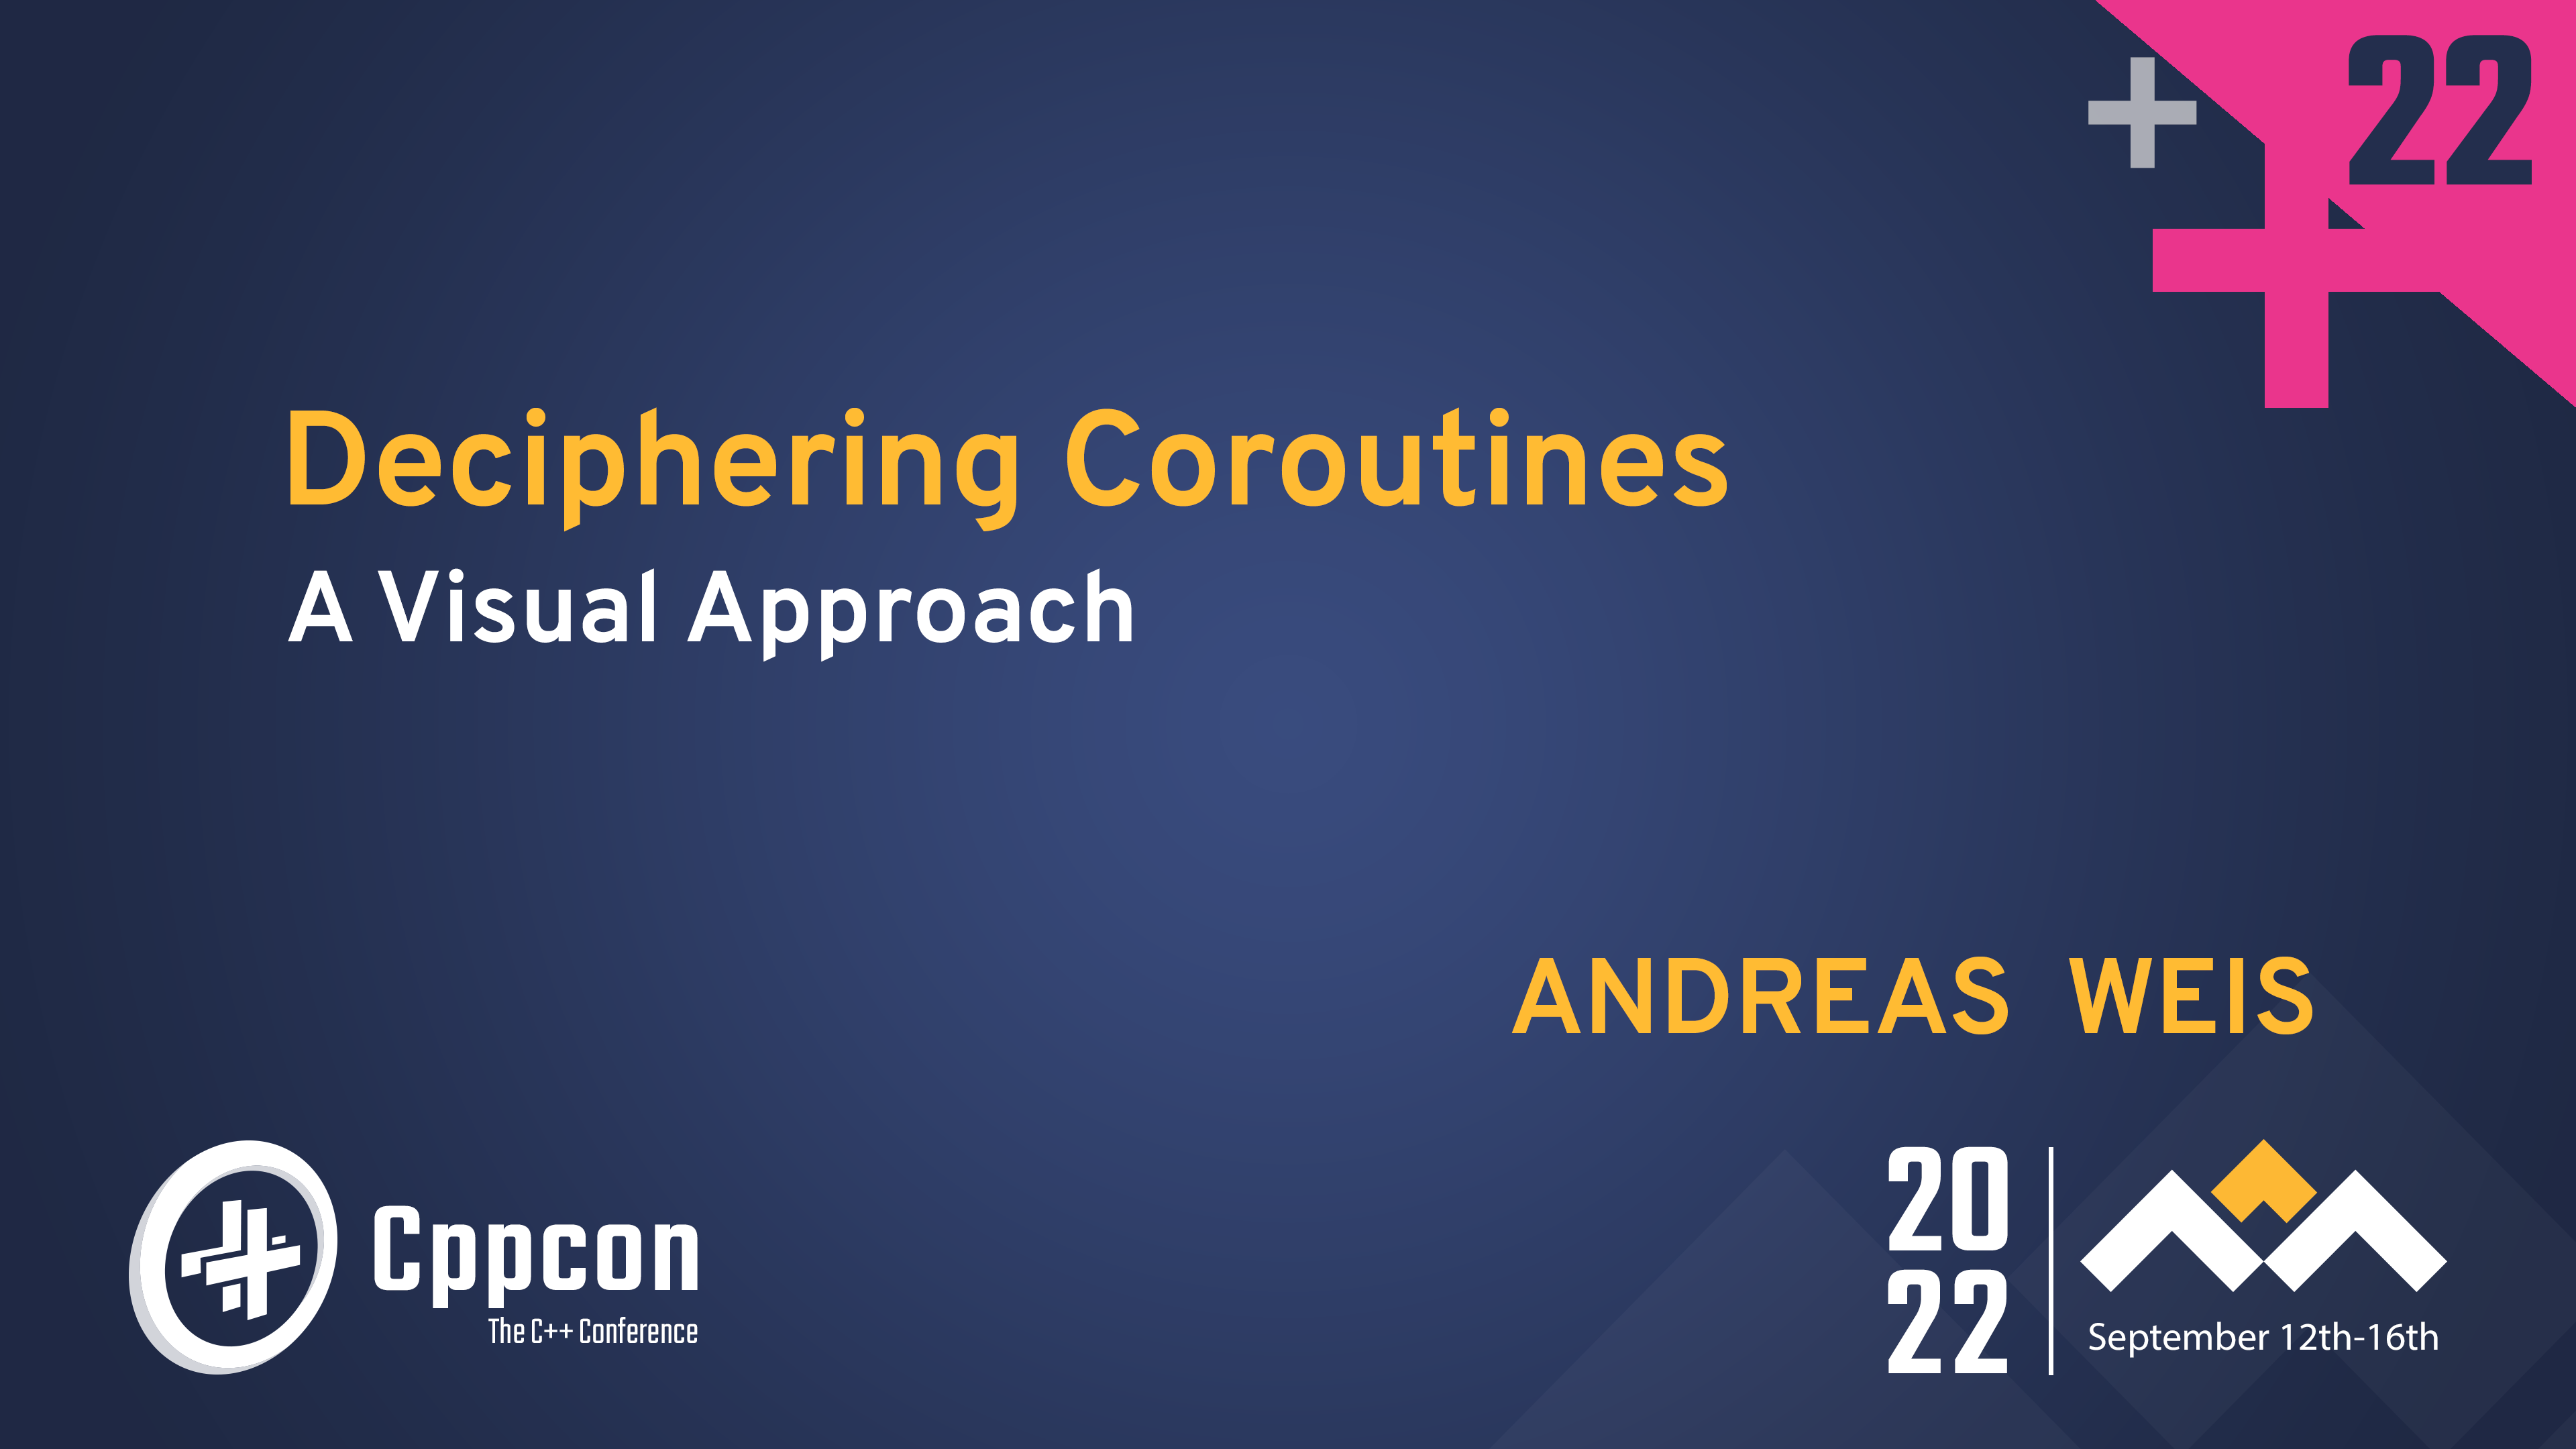
\includegraphics[keepaspectratio,
                                 width=\paperwidth,
                                 height=\paperheight]{corogfx/cppcon_titlecard.png}
            };
        \end{tikzpicture}
     \end{frame}
}

\frame{\titlepage}

\iftrue %crop
\fi

\begin{frame}[fragile]
  \frametitle{About me - Andreas Weis (he/him)}

  \begin{itemize}
    \setlength\itemsep{1.5em}

    \item \href{https://stackoverflow.com/users/577603/comicsansms}{
\includegraphics[height=.05\textheight]{resources/so-icon.png}} \href{https://github.com/ComicSansMS}{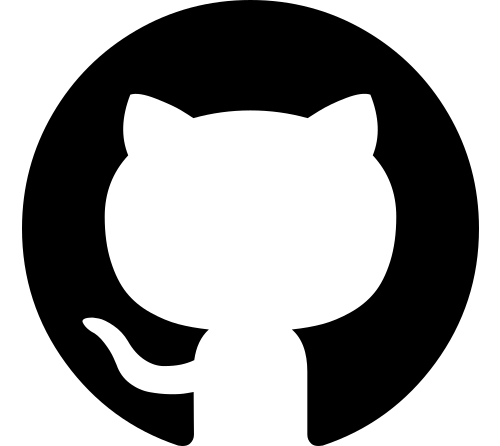
\includegraphics[height=.05\textheight]{resources/github-icon.png}} \includegraphics[height=.05\textheight]{resources/discord-icon.png} ComicSansMS

    \item \href{https://twitter.com/DerGhulbus/}{
\includegraphics[height=.05\textheight]{resources/twitter-icon.png} @DerGhulbus}

    \item 
\includegraphics[height=.05\textheight]{resources/meetup-icon.png} Co-organizer of the \href{https://www.meetup.com/MUCplusplus/}{Munich C++ User Group}

    \item Currently working as a Runtime Engineer for Woven Planet 
\includegraphics[height=.1\textheight]{resources/Woven_Planet_Holdings_Logo.png}

  \end{itemize}
\end{frame}

\begin{frame}
  \frametitle{Motivation}
  
  \begin{center}
  Coroutines are hard!
  \end{center}
  
  \note{
  \begin{itemize}
  \item Coroutines are hard
  \item Allow for extremely complex transformations of control flow
  \item Use an arcane syntax that changes some of the fundamental language rules 
  \item Hard to understand, but even harder to remember when not used regularly
  \item Idea of the talk is to introduce them in a way that you can remember easily
  \item Feature is too big to introduce all at once; focus only on syntax
  \end{itemize}
  }
\end{frame}

\begin{frame}
  \frametitle{Overview}
  \begin{itemize}
    \item Essential use cases for coroutines
    \item Coroutines from the caller's perspective
    \item Steps involved in starting a coroutine
    \item Suspend and resume
    \item Drawing a map of coroutine land
    \item Interacting with coroutines
    \end{itemize}
\end{frame}

%\iffalse %!!!!!!!!!!!!!!!!!

\begin{frame}
  \frametitle{Disclaimer}
  
  \note{
  \begin{itemize}
    \item Coroutines are extremely powerful and flexible.
    \item For didactic reasons we will simplify things in places and ignore some of the more advanced features to keep explanations streamlined.
    \item Please keep in mind that this all code on the slides is meant to illustrate specific relationships in a simplified way and should not be taken as best practices for writing coroutine code.
  \end{itemize}
  }
\end{frame}

\begin{frame}
  \frametitle{Coroutine Basics}
  
  \begin{center}
  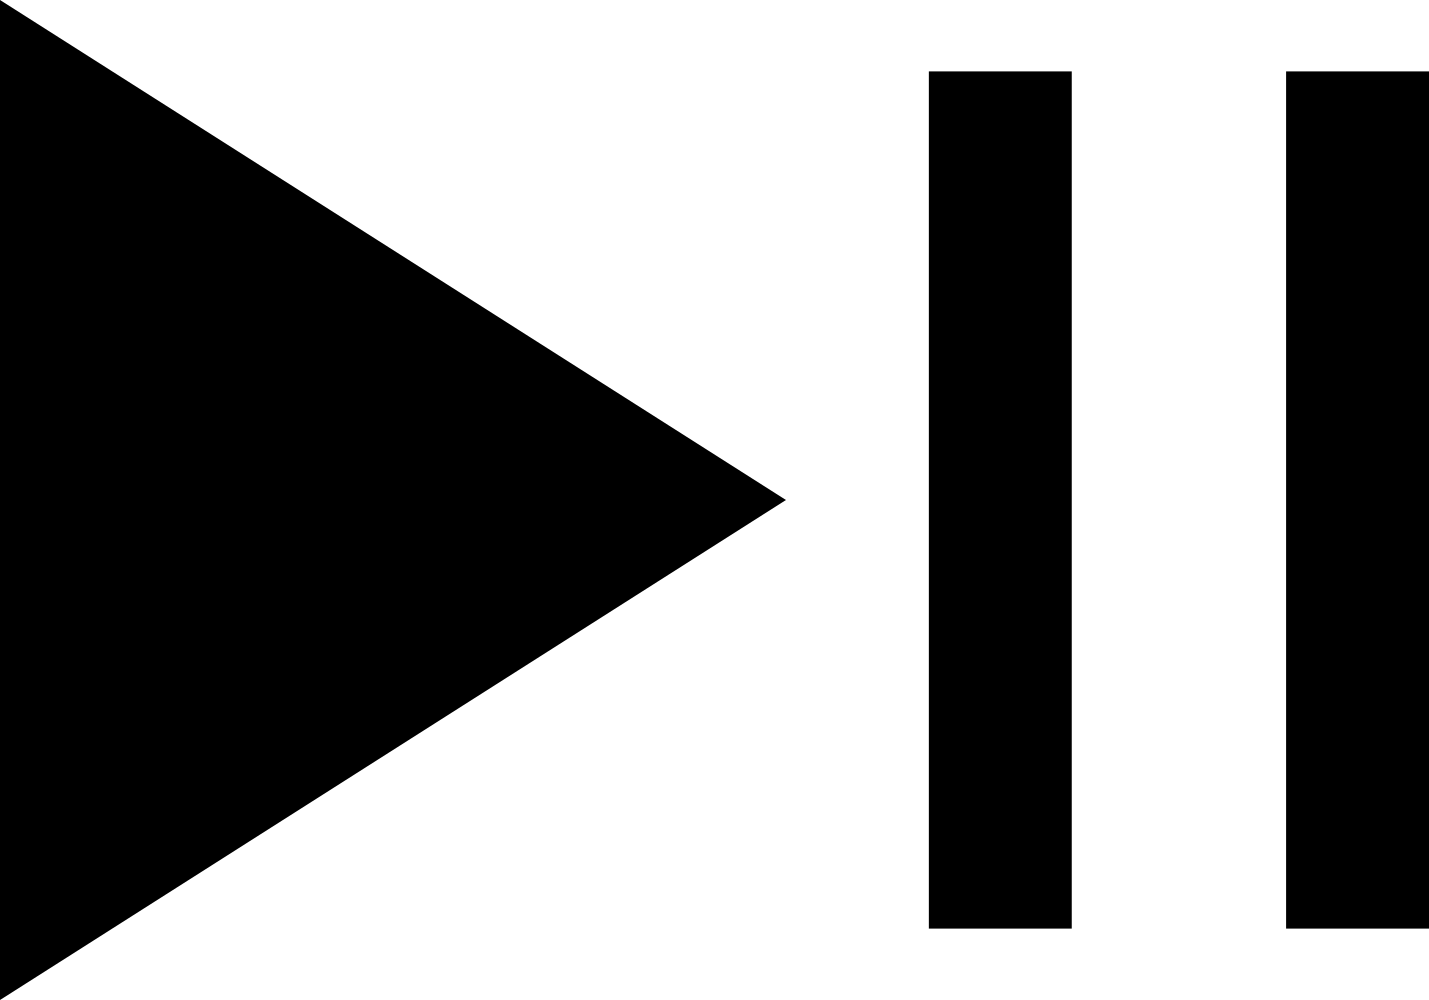
\includegraphics[height=.75\textheight]{corogfx/icon_play_pause.png}
  \end{center}
  
  \note{
  \begin{itemize}
    \item Function that can be paused
    \item Can be resumed later with surrounding state still intact
    \item Coroutine is always stateful - we need to remember where we left off
    \item Think of coroutines like factory functions returning a function object
    \item Stackless
  \end{itemize}
  }
\end{frame}

\begin{frame}[fragile]
  \frametitle{Coroutine Basics - Asynchronous computation}

  \begin{lstlisting}[language={C++}]
auto [ec, bytes_read] = read(socket, buffer);
// ...

async_read(socket, buffer,
  [](std::error_code ec, std::size_t bytes_read) {
    // ...
  });
  \end{lstlisting}
\end{frame}

\begin{frame}[fragile]
  \frametitle{Coroutine Basics - Asynchronous computation}

  \begin{lstlisting}[language={C++}]
auto [ec, bytes_read] = read(socket, buffer);
// ...

auto [ec, bytes_read] =
         co_await async_read(socket, buffer);
// ...
  \end{lstlisting}
\end{frame}

\begin{frame}[fragile]

\frametitle{Coroutine Basics - Suspend/resume}

  \begin{lstlisting}[language={C++}]
MyCoroutine co = startComputation(initial_data);
auto some_results = co.provide(some_data);
auto more_results = co.provide(more_data);
auto final_results = co.results;
  \end{lstlisting}
\end{frame}


\begin{frame}[fragile]
  \frametitle{A simple example}
  
  \begin{lstlisting}[style=cpp20]
// Returns a vector containing the first n
// elements of the Fibonacci series:
// 1, 1, 2, 3, 5, 8, 13, 21, ...

std::vector<int> fibo(int n);
  \end{lstlisting}
  
  \note{
  \begin{itemize}
    \item We start with a simple function
    \item Generates a series of numbers
    \item Naïve implementation returning a vector containing the series
    \item Disadvantages?
    \item Requires O(n) storage
    \item Doesn't work for infinite ranges
  \end{itemize}
  }
\end{frame}

\begin{frame}[fragile]
  \frametitle{A simple example}
  
  \begin{lstlisting}[style=cpp20]
class FiboGenerator {
  // Successive calls to next() return the
  //  numbers from the Fibonacci series
  // 1, 1, 2, 3, 5, 8, 13, 21, ...
  int next();
};

// Returns a new FiboGenerator object that 
// will start from the first Fibonacci number
(*@\tikz[baseline,inner sep=0]\node[anchor=base](nom1){};@*)FiboGenerator(*@\tikz[baseline,inner sep=0]\node[anchor=base](nom2){};@*) makeFiboGenerator();
  \end{lstlisting}
  \iftransitions \pause \fi Is \texttt{makeFiboGenerator()} a coroutine?
  \iftransitions \pause \fi \tikz[overlay]\filldraw[blue, opacity=0.3] (nom1) rectangle ([shift={(0,2ex)}]nom2);
  
  \note{
  \begin{itemize}
    \item Alternative approach: Return a generator object which produces the numbers lazily
    \item Interesting functionality now moved to the next() function
    \item TRANSITION Is makeFiboGenerator() a coroutine?
    \item Maybe. We don't know. All we see is the interface.
    \item TRANSITION The first important part of writing a coroutine: The return object
  \end{itemize}
  }
\end{frame}

\begin{frame}

\frametitle{The coroutine return type}

\begin{center}
\tikz \draw node[pos=.5,fill=co_return_object,scale=4] {ReturnType};

\note{Timecheck: 0:10}
\end{center}

  \note{
  \begin{itemize}
    \item The initial call to a coroutine typically returns an object back to the user representing the its state
    \item The interface of this coroutine object determines how a client interacts with the coroutine
    \item But the fact that it is implemented as a coroutine is an implementation detail; no way to tell from the outside
    \item Client does not need to know anything about coroutines, they just need to understand the interface of the return object; no special rules
    \item Important: WE decide what the return type interface looks like. Wide range of possibilities.
  \end{itemize}
  }
\end{frame}


\begin{frame}
    \frametitle{What turns a function into a coroutine?}
    
    \iftransitions \pause \fi

    If it makes use of either of the three keywords
    \begin{itemize}
    \item \texttt{co\_await}
    \item \texttt{co\_return}
    \item \texttt{co\_yield}
    \end{itemize}
    
  \note{
  \begin{itemize}
    \item What turns a function into a coroutine?
    \item We can't tell from its signature, so how does the compiler know.
    \item TRANSITION One of the keywords has to appear in the body
    \item If you see one of those in a function body you're dealing with a coroutine
    \item This drastically changes the language rules for the body
    \item For instance, you can't use plain return in a coroutine
  \end{itemize}
  }
\end{frame}

\begin{frame}[fragile]
  \frametitle{The body of \texttt{makeFiboGenerator}}
  
  \begin{lstlisting}[style=cpp20]
FiboGenerator makeFiboGenerator() {
  int i1 = 1;
  int i2 = 1;
  while (;;) {
    co_yield i1;
    i1 = std::exchange(i2, i1 + i2);
  }
}
  \end{lstlisting}

  \note{
  \begin{itemize}
    \item The body of makeFiboGenerator
    \item This looks a lot like the naïve implementation for filling the vector
    \item But the signature does not match the implementation at all
    \item The rest of the talk we will try to understand the special rules for the coroutine function body
  \end{itemize}
  }
\end{frame}


\begin{frame}[fragile]
  \frametitle{The smallest coroutine}
  
  \iftransitions \pause \fi
  \begin{lstlisting}[style=cpp20]
(*@\tikz[baseline,inner sep=0]\node[anchor=base](ar01){};@*)ReturnType(*@\tikz[baseline,inner sep=0]\node[anchor=base](br01){};@*) hello_coroutine() {
  co_return;
}
  \end{lstlisting}

  \iftransitions \pause \fi \tikz[overlay]\filldraw[blue, opacity=0.3] ([shift={(0,-0.5ex)}]ar01) rectangle ([shift={(0,2ex)}]br01);

  \note{
  \begin{itemize}
    \item Let's start the small. What is the simplest possible coroutine?
    \item TRANSITION The smallest possible coroutine. Empty body, but we need co\_return to turn it into a coroutine
    \item TRANSITION This is going to be our return object, so let's implement it
  \end{itemize}
  }
\end{frame}

\begin{frame}[fragile]

  \frametitle{Implementing the return object}

  \begin{lstlisting}[style=cpp20]
struct ReturnType {
};
  \end{lstlisting}
  
  \iftransitions \pause \fi
  
  \vfill
  
  Compiler Error: Compiler is looking for a nested type \texttt{ReturnType::promise\_type}.
  
  \note{
  \begin{itemize}
    \item Let's see what happens with an empty type
    \item TRANSITION: Compiler error, missing promise
  \end{itemize}
  }
\end{frame}

\begin{frame}[fragile]

  \frametitle{Implementing the return object}

  \begin{lstlisting}[style=cpp20]
struct ReturnType {
  struct (*@\tikz[baseline,inner sep=0]\node[anchor=base](ar02){};@*)promise_type(*@\tikz[baseline,inner sep=0]\node[anchor=base](br02){};@*) {};
};
  \end{lstlisting}

  \iftransitions \pause \fi \tikz[overlay]\filldraw[red, opacity=0.3] ([shift={(0,-0.5ex)}]ar02) rectangle ([shift={(0,2ex)}]br02);
  
  \note{
  \begin{itemize}
    \item So we need to provide the promise as well
    \item We do it inline, could also be a typedef
    \item TRANSITION: Introducing the second important participant in the coroutine mechanism
  \end{itemize}
  }
\end{frame}


\begin{frame}
\frametitle{The coroutine promise}

\begin{center}
\tikz \draw node[pos=.5,fill=co_promise,scale=4] {promise\_type};
\end{center}

  \note{
  Timecheck: 0:18
  \begin{itemize}
    \item Why do we need the promise? Return object is like future, given to caller. Promise is the promise that resides in the producer
    \item Main point of interaction from within the coroutine
    \item Unlike future promise, this one is special and gets constructed by the compiler
    \item Promise is the central intersection point for coroutine and caller
    \item Determines what happens at essential points in a coroutines lifetime: Start and completion of execution; exit via \texttt{co\_return} or exception
  \end{itemize}
  }
\end{frame}

\iftransitions
\begin{frame}[fragile]
  \frametitle{Implementing the promise}
  
  \setbeamercolor{alerted text}{fg=red}
  \setbeamerfont{alerted text}{series=\bfseries,family=\ttfamily}
  
  \begin{semiverbatim}
{\color{blue}struct} promise_type \{
  
  \uncover<2->{\alert<2>{ReturnType get_return_object() \{ {\color{blue}return} \{\}; \}}}
  \uncover<5->{\alert<5>{std::suspend_always initial_suspend() \{ {\color{blue}return} \{\}; \}}}
  
  \uncover<3->{\alert<3>{void return_void() \{ \}}}
  \uncover<4->{\alert<4>{void unhandled_exception() \{ \};}}
  \uncover<5->{\alert<5>{std::suspend_always final_suspend() noexcept \{ {\color{blue}return} \{\}; \}}}
  
\};
  \end{semiverbatim}
  
  \uncover<3->{ \tikz[overlay]\filldraw[blue, opacity=0.3] (1em,4.9) rectangle ++ (5.5em,-0.4); }
  
  \note {
  What goes inside the promise? ...
  \begin{itemize}
    \item TRANSITION get\_return\_object
    \item TRANSITION return\_void / return\_value
    \item TRANSITION unhandled except; all the return paths
    \item TRANSITION suspend - when is it called. we don't understand yet what it does.
  \end{itemize}
  
  }
\end{frame}
\else
\begin{frame}[fragile]
  \frametitle{Implementing the promise}

  \begin{semiverbatim}
{\color{blue}struct} promise_type \{
  
  ReturnType get_return_object() \{ {\color{blue}return} \{\}; \}
  std::suspend_always initial_suspend() \{ {\color{blue}return} \{\}; \}
  
  void return_void() \{ \}
  void unhandled_exception() \{ \};
  std::suspend_always final_suspend() noexcept \{ {\color{blue}return} \{\}; \}
  
\};
  \end{semiverbatim}
  
  \tikz[overlay]\filldraw[blue, opacity=0.3] (1em,4.9) rectangle ++ (5.5em,-0.4);
\end{frame}
\fi

\begin{frame}[fragile]

  \frametitle{Running the code}

  \begin{semiverbatim}
\alert<2>{std::suspend_always} initial_suspend() \{ return \{ \}; \}
  \end{semiverbatim}

  \begin{lstlisting}[style=cpp20]
ReturnType hello_coroutine() {
  std::println("Hello from coroutine!");
  co_return;
}

int main() {
  hello_coroutine();    // prints nothing
}
\end{lstlisting}

  \note {
    Leaks the coroutine frame!
  }

\end{frame}


\begin{frame}[fragile]

  \frametitle{Running the code}

  \begin{semiverbatim}
\alert<1>{std::suspend_never}  initial_suspend() \{ return \{ \}; \}
  \end{semiverbatim}

  \begin{lstlisting}[style=cpp20]
ReturnType hello_coroutine() {
  std::println("Hello from coroutine!");
  co_return;
}

int main() {
  hello_coroutine();    // prints "Hello from coroutine!"
}
\end{lstlisting}


\end{frame}

\begin{frame}

  \frametitle{Coroutine Suspension}
  
  \begin{center}
  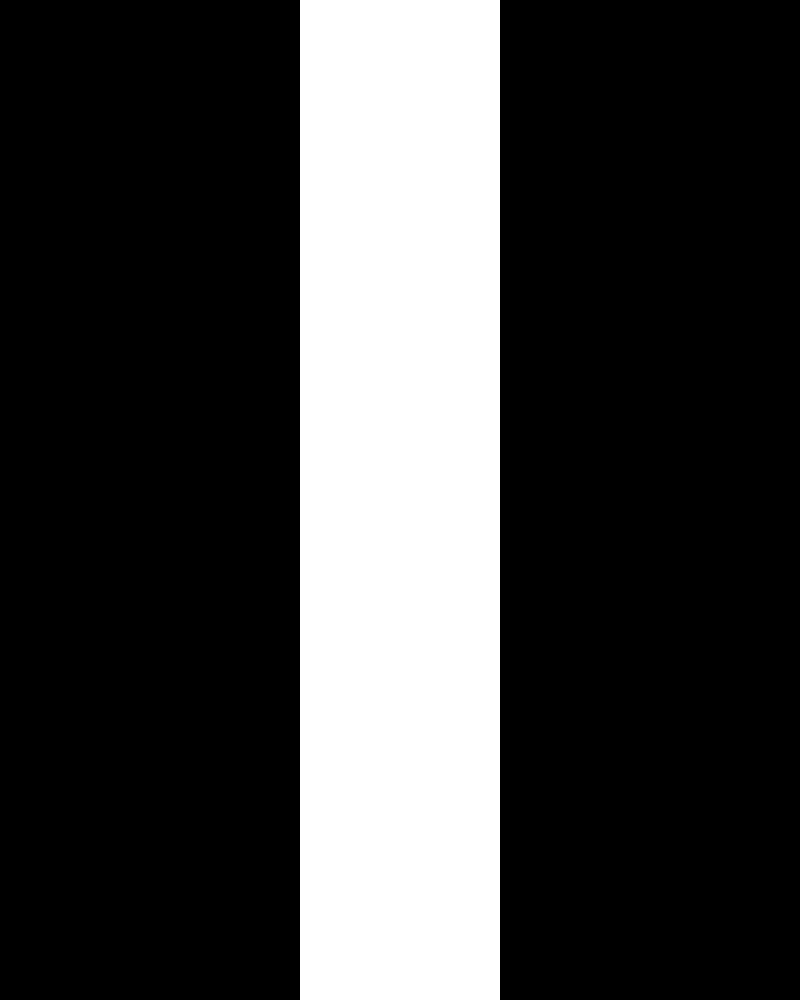
\includegraphics[height=.75\textheight]{corogfx/icon_pause.png}
  \end{center}

\end{frame}

\begin{frame}

  \frametitle{Awaitable}
  
  \begin{center}
  \tikz \draw node[pos=.5,fill=co_awaitable,scale=4] {Awaitable};
  \end{center}

  \note{Timecheck: 0:25}
\end{frame}

\begin{frame}[fragile]
  \frametitle{Awaitable}
  
  \begin{lstlisting}[style=cpp20]
(*@\tikz[baseline,inner sep=0]\node[anchor=base](ar06){};@*)AsyncRead(*@\tikz[baseline,inner sep=0]\node[anchor=base](br06){};@*) awaitable = async_read(socket, buffer);
auto [ec, bytes_read] = co_await awaitable;
  \end{lstlisting}
  
  \tikz[overlay]\filldraw[green, opacity=0.3] ([shift={(0,-0.5ex)}]ar06) rectangle ([shift={(0,2ex)}]br06);
  
  \note{
  \begin{itemize}
    \item A type that can be co\_awaited on
    \item An opportunity for suspension
    \item Provides a hook to inject code into suspend resume, just like promise provided hooks for start/stop
    \item May decide not to suspend at all
  \end{itemize}
  }

\end{frame}

\iftransitions
\begin{frame}[fragile]
  \frametitle{Implementing the awaitable}
  
  \setbeamercolor{alerted text}{fg=red}
  \setbeamerfont{alerted text}{series=\bfseries,family=\ttfamily}
  
  \begin{semiverbatim}
{\color{blue}struct} Awaitable \{
  \uncover<2->{\alert<2>{{\color{blue}bool} await_ready();}}
  \uncover<3-3>{\alert<3>{{\color{blue}void} await_suspend(std::coroutine_handle <>);}}

\};
  \end{semiverbatim}
  
  \uncover<1->{ \tikz[overlay]\filldraw[red, opacity=0] (23.15em,2.5) rectangle ++ (6.2em,-0.4); }
\end{frame}
\fi

\iftransitions
\begin{frame}[fragile]
  \frametitle{Implementing the awaitable}
  
  \setbeamercolor{alerted text}{fg=red}
  \setbeamerfont{alerted text}{series=\bfseries,family=\ttfamily}
  
  \begin{semiverbatim}
{\color{blue}struct} Awaitable \{
  {\color{blue}bool} await_ready();
  \uncover<1->{{\color{blue}void} await_suspend(std::coroutine_handle <\alert<1>{promise_type}>);}
  \uncover<3-4>{\alert<3>{{\color{blue}void} await_resume();}}
\};
  \end{semiverbatim}
  
  \uncover<2->{ \tikz[overlay]\filldraw[red, opacity=0.3] (23.15em,2.5) rectangle ++ (6.2em,-0.4); }
\end{frame}
\else
\begin{frame}[fragile]
  \frametitle{Implementing the awaitable}

  \begin{semiverbatim}
{\color{blue}struct} Awaitable \{
  {\color{blue}bool} await_ready();
  {\color{blue}void} await_suspend(std::coroutine_handle promise_type>);
  {\color{blue}void} await_resume();
\};
  \end{semiverbatim}
  
  \tikz[overlay]\filldraw[red, opacity=0.3] (22.5em,2.5) rectangle ++ (6.4em,-0.4);
\end{frame}
\fi

\begin{frame}[fragile]
  \frametitle{The simplest awaitable}
  
  \begin{lstlisting}[style=cpp20]
struct SuspendAlways {
  bool await_ready() { return false; }
  void await_suspend(std::coroutine_handle<>) {}
  void await_resume() {}
};
  \end{lstlisting}
\end{frame}


\begin{frame}[fragile]

  \frametitle{Coroutine handle interface}
  
  \begin{lstlisting}[style=cpp20]
struct std::coroutine_handle<promise_type> {
  // ...
  void resume() const; (*@ \iftransitions \pause \fi @*)
  void destroy() const; (*@ \iftransitions \pause \fi @*)
  promise_type& promise() const;
  static coroutine_handle from_promise(promise_type&); 
};
  \end{lstlisting}

\end{frame}


\iffalse

\begin{frame}
  \frametitle{Order of events on Coroutine startup}

  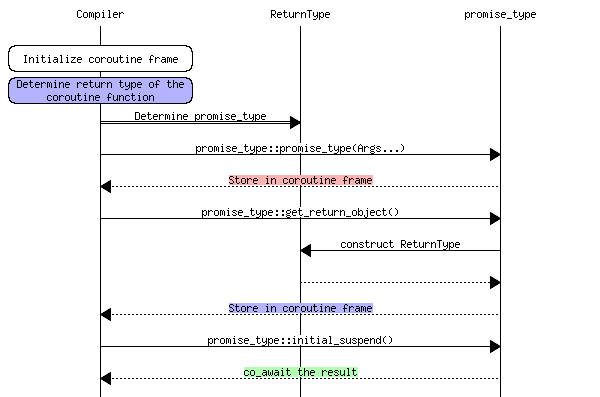
\includegraphics[height=.9\textheight]{corogfx/start_flow.png}
\end{frame}

\begin{frame}
  \frametitle{Order of events on Coroutine stop}

  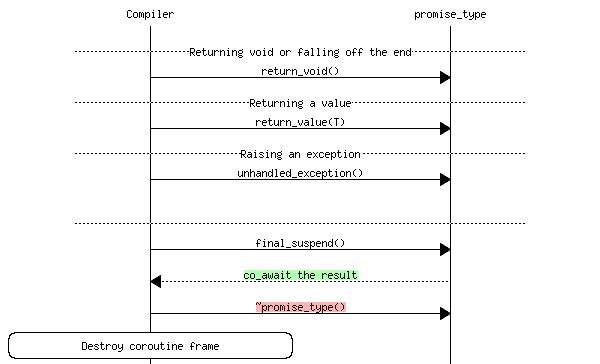
\includegraphics[height=.9\textheight]{corogfx/stop_flow.png}
\end{frame}

\fi


\iffalse
\begin{frame}[fragile]

  \frametitle{Promise Cheat Sheet}

  \begin{lstlisting}[style=cpp20]
struct ReturnType {
  struct promise_type {
    promise_type(T...);
    ReturnType get_return_object();
    std::suspend_always initial_suspend();
    // ---- (*@$\Uparrow$@*) Start / (*@$\Downarrow$@*) Shutdown ----
    void return_void();
    void return_value(T);
    void unhandled_exception();
    std::suspend_always final_suspend() noexcept;
  };
};
  \end{lstlisting}
  
  \note{Timecheck: 0:30}
\end{frame}
\fi

\begin{frame}[fragile]

  \frametitle{Cheat Sheet - Start/Stop}

  \begin{lstlisting}[style=cpp20,numbers=left]
struct (*@\tikz[baseline,inner sep=0]\node[anchor=base](ar100){};@*)ReturnType(*@\tikz[baseline,inner sep=0]\node[anchor=base](br100){};@*) / std::coroutine_traits<(*@\tikz[baseline,inner sep=0]\node[anchor=base](mr100){};@*)ReturnType(*@\tikz[baseline,inner sep=0]\node[anchor=base](nr100){};@*), ...> { 
  struct (*@\tikz[baseline,inner sep=0]\node[anchor=base](cr100){};@*)promise_type(*@\tikz[baseline,inner sep=0]\node[anchor=base](dr100){};@*) {
    (*@\tikz[baseline,inner sep=0]\node[anchor=base](kr100){};@*)promise_type(T...);(*@\tikz[baseline,inner sep=0]\node[anchor=base](lr100){};@*)  // opt.
    (*@\tikz[baseline,inner sep=0]\node[anchor=base](er100){};@*)ReturnType(*@\tikz[baseline,inner sep=0]\node[anchor=base](fr100){};@*) get_return_object();
    (*@\tikz[baseline,inner sep=0]\node[anchor=base](gr100){};@*)std::suspend_always(*@\tikz[baseline,inner sep=0]\node[anchor=base](hr100){};@*) initial_suspend();
    // ---- (*@$\Uparrow$@*) Start / (*@$\Downarrow$@*) Shutdown ----
    void return_value(T); / void return_void();
    void unhandled_exception();
    (*@\tikz[baseline,inner sep=0]\node[anchor=base](ir100){};@*)std::suspend_always(*@\tikz[baseline,inner sep=0]\node[anchor=base](jr100){};@*) final_suspend() noexcept;
\end{lstlisting}\begin{lstlisting}[style=cpp20]
  };
};
  \end{lstlisting}
  
  \tikz[overlay]\filldraw[blue, opacity=0.3] ([shift={(0,-0.5ex)}]ar100) rectangle ([shift={(0,2ex)}]br100);
  \tikz[overlay]\filldraw[blue, opacity=0.3] ([shift={(0,-0.5ex)}]mr100) rectangle ([shift={(0,2ex)}]nr100);
  \tikz[overlay]\filldraw[red, opacity=0.3] ([shift={(0,-0.5ex)}]cr100) rectangle ([shift={(0,2ex)}]dr100);
  %\tikz[overlay]\filldraw[red, opacity=0.3] ([shift={(0,-0.5ex)}]kr100) rectangle ([shift={(0,2ex)}]lr100);
  \tikz[overlay]\filldraw[blue, opacity=0.3] ([shift={(0,-0.5ex)}]er100) rectangle ([shift={(0,2ex)}]fr100);
  \tikz[overlay]\filldraw[green, opacity=0.3] ([shift={(0,-0.5ex)}]gr100) rectangle ([shift={(0,2ex)}]hr100);
  \tikz[overlay]\filldraw[green, opacity=0.3] ([shift={(0,-0.5ex)}]ir100) rectangle ([shift={(0,2ex)}]jr100);
\end{frame}

\begin{frame}[fragile]

  \frametitle{Cheat Sheet - Awaitable}

  \begin{lstlisting}[style=cpp20,numbers=left]
struct (*@\tikz[baseline,inner sep=0]\node[anchor=base](ar101){};@*)Awaitable(*@\tikz[baseline,inner sep=0]\node[anchor=base](br101){};@*) {
  bool await_ready();
  void await_suspend(std::coroutine_handle <(*@\tikz[baseline,inner sep=0]\node[anchor=base](cr101){};@*)promise_type(*@\tikz[baseline,inner sep=0]\node[anchor=base](dr101){};@*)>);
  void await_resume(); 
};
\end{lstlisting}
  
  \tikz[overlay]\filldraw[green, opacity=0.3] ([shift={(0,-0.5ex)}]ar101) rectangle ([shift={(0,2ex)}]br101);
  \tikz[overlay]\filldraw[red, opacity=0.3] ([shift={(0,-0.5ex)}]cr101) rectangle ([shift={(0,2ex)}]dr101);
\end{frame}

\begin{frame}

  \frametitle{The key components}
  
  \begin{itemize}
  \item Return Type
  \item Promise Type
  \item Awaitable Type
  \item \texttt{std::coroutine\_handle<>}
  \end{itemize}
\end{frame}

\begin{frame}

  \frametitle{Resuming}
  
  \begin{center}
  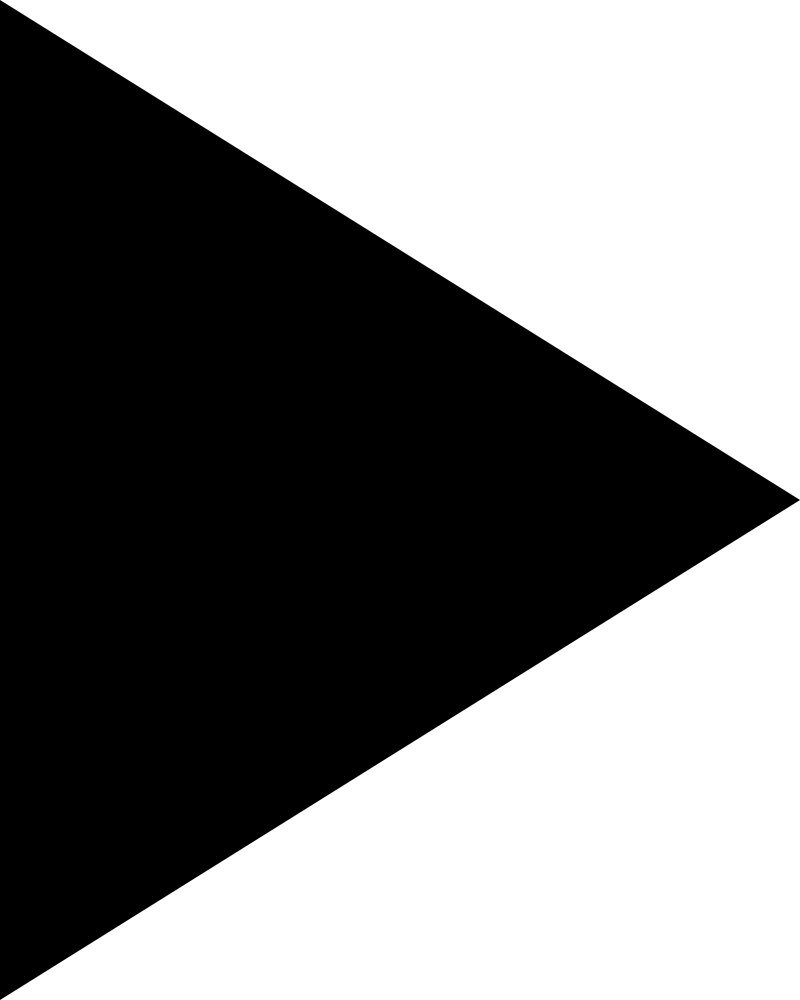
\includegraphics[height=.75\textheight]{corogfx/icon_play.png}
  \end{center}

\end{frame}

\begin{frame}[fragile]

  \frametitle{Back to Hello World}

%\begin{tikzpicture}[overlay]
%  \draw (15,0) circle [radius=2pt];
%  \node[draw,minimum width=10em] at (10,-2) {main 1};
%\end{tikzpicture}

  \begin{semiverbatim}
\alert<1>{std::suspend_always} initial_suspend() \{ return \{ \}; \}
  \end{semiverbatim}

  \begin{lstlisting}[style=cpp20]
ReturnType hello_coroutine() {
  std::println("Hello from coroutine!");
  co_return;
}

int main() {
  ReturnType c = hello_coroutine();    // prints nothing
  c.resume();         // prints "Hello from coroutine!"
}
\end{lstlisting}

\note {
  Resumption is triggered via coroutine\_handle
  
  But how do we get to the handle from inside ReturnType::resume?
}
\end{frame}

\begin{frame}[fragile]
  \frametitle{Making acquaintances}
  
  \begin{center}
  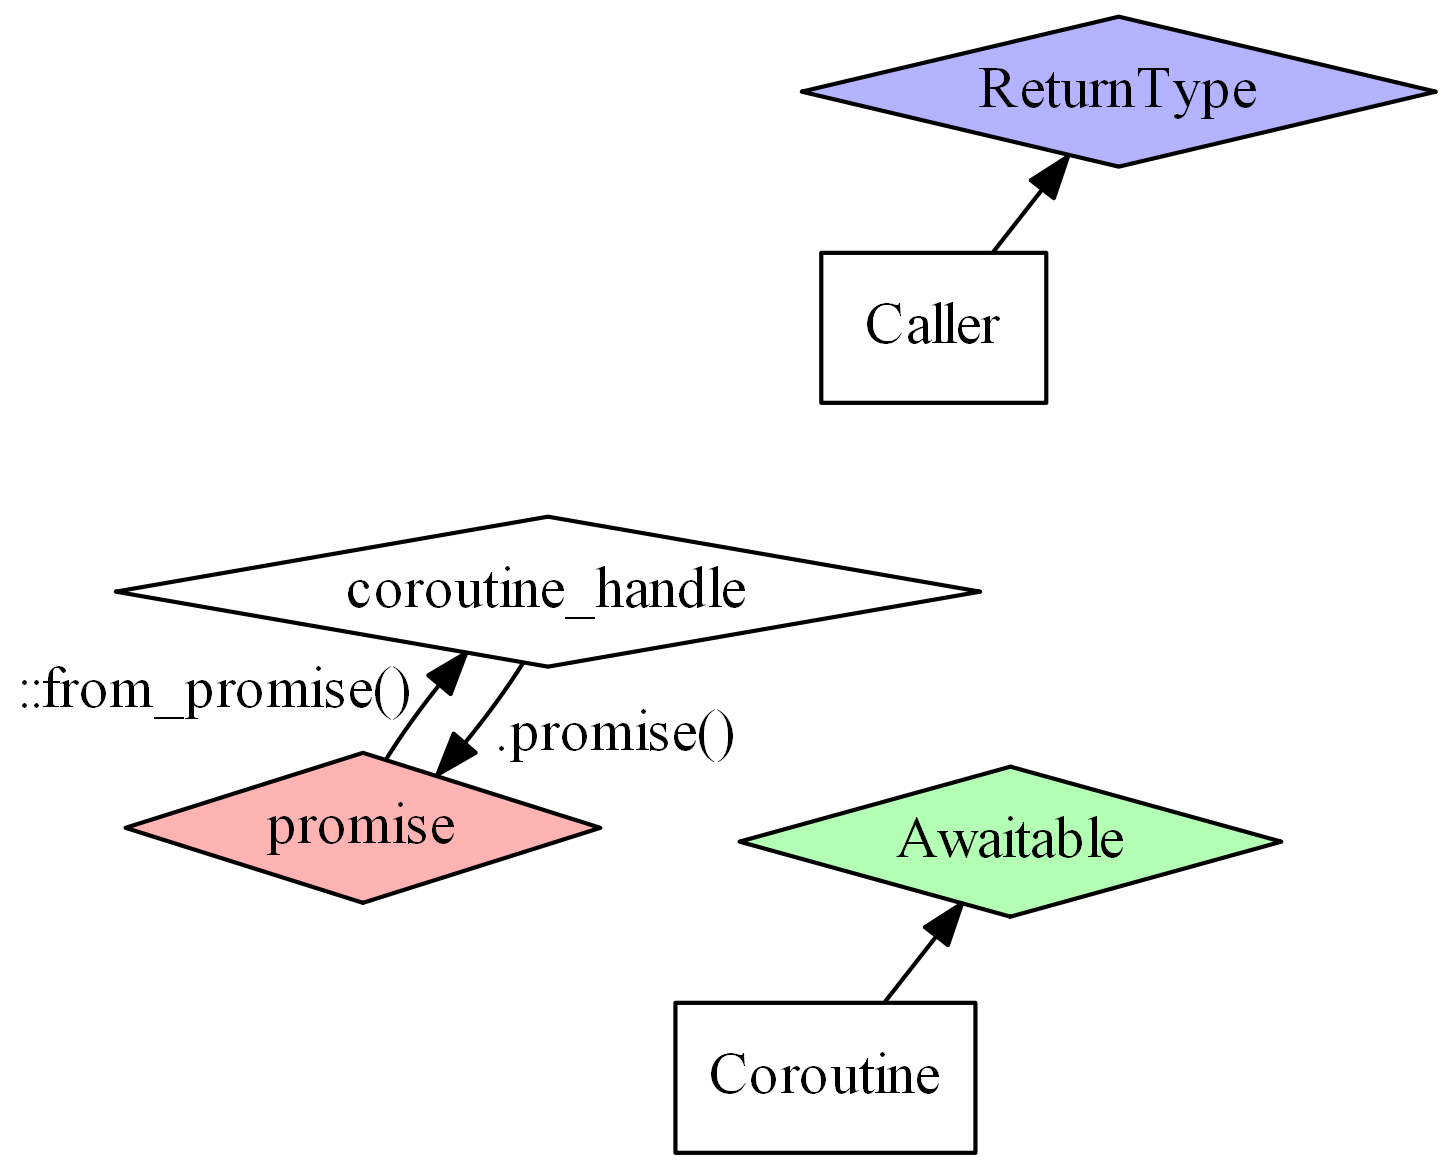
\includegraphics[height=.9\textheight]{corogfx/acquaintances01.png}
  \end{center}
\end{frame}

\begin{frame}[fragile]
  \frametitle{Making acquaintances}

  \begin{lstlisting}[style=cpp20]
struct (*@\tikz[baseline,inner sep=0]\node[anchor=base](cr07){};@*)promise_type(*@\tikz[baseline,inner sep=0]\node[anchor=base](dr07){};@*) {
  (*@\tikz[baseline,inner sep=0]\node[anchor=base](er07){};@*)ReturnType(*@\tikz[baseline,inner sep=0]\node[anchor=base](fr07){};@*) get_return_object();
};
  \end{lstlisting}
  
  \tikz[overlay]\filldraw[blue, opacity=0.3] ([shift={(0,-0.5ex)}]er07) rectangle ([shift={(0,2ex)}]fr07);
  \tikz[overlay]\filldraw[red, opacity=0.3] ([shift={(0,-0.5ex)}]cr07) rectangle ([shift={(0,2ex)}]dr07);
\end{frame}

\begin{frame}[fragile]
  \frametitle{Making acquaintances}

  \begin{lstlisting}[style=cpp20]
struct (*@\tikz[baseline,inner sep=0]\node[anchor=base](cr07){};@*)promise_type(*@\tikz[baseline,inner sep=0]\node[anchor=base](dr07){};@*) {
  (*@\tikz[baseline,inner sep=0]\node[anchor=base](er07){};@*)ReturnType(*@\tikz[baseline,inner sep=0]\node[anchor=base](fr07){};@*) get_return_object() {
      return ReturnType{
        std::coroutine_handle<promise>::from_promise(*this)
      };
  }
};
  \end{lstlisting}
  
  \tikz[overlay]\filldraw[blue, opacity=0.3] ([shift={(0,-0.5ex)}]er07) rectangle ([shift={(0,2ex)}]fr07);
  \tikz[overlay]\filldraw[red, opacity=0.3] ([shift={(0,-0.5ex)}]cr07) rectangle ([shift={(0,2ex)}]dr07);
\end{frame}

\begin{frame}[fragile]
  \frametitle{Making acquaintances}

  \begin{lstlisting}[style=cpp20]
struct (*@\tikz[baseline,inner sep=0]\node[anchor=base](cr07){};@*)promise_type(*@\tikz[baseline,inner sep=0]\node[anchor=base](dr07){};@*) {
  (*@\tikz[baseline,inner sep=0]\node[anchor=base](er07){};@*)ReturnType(*@\tikz[baseline,inner sep=0]\node[anchor=base](fr07){};@*) get_return_object()
    return ReturnType{
      std::coroutine_handle<promise>::from_promise(*this)
      };
  }
};
struct (*@\tikz[baseline,inner sep=0]\node[anchor=base](ar07){};@*)ReturnType(*@\tikz[baseline,inner sep=0]\node[anchor=base](br07){};@*) {
  std::coroutine_handle<promise_type> handle;
  ReturnType(std::coroutine_handle<promise_type> h)
  : handle(h) {}
  void resume() { handle.resume(); }
};
  \end{lstlisting}
  
  \tikz[overlay]\filldraw[blue, opacity=0.3] ([shift={(0,-0.5ex)}]ar07) rectangle ([shift={(0,2ex)}]br07);
  \tikz[overlay]\filldraw[red, opacity=0.3] ([shift={(0,-0.5ex)}]cr07) rectangle ([shift={(0,2ex)}]dr07);
  \tikz[overlay]\filldraw[blue, opacity=0.3] ([shift={(0,-0.5ex)}]er07) rectangle ([shift={(0,2ex)}]fr07);
  
  \note {
  When suspending on initial\_suspend, handle must be stored somewhere
  }
\end{frame}

\begin{frame}[fragile]
  \frametitle{Making acquaintances}
  
  \begin{center}
  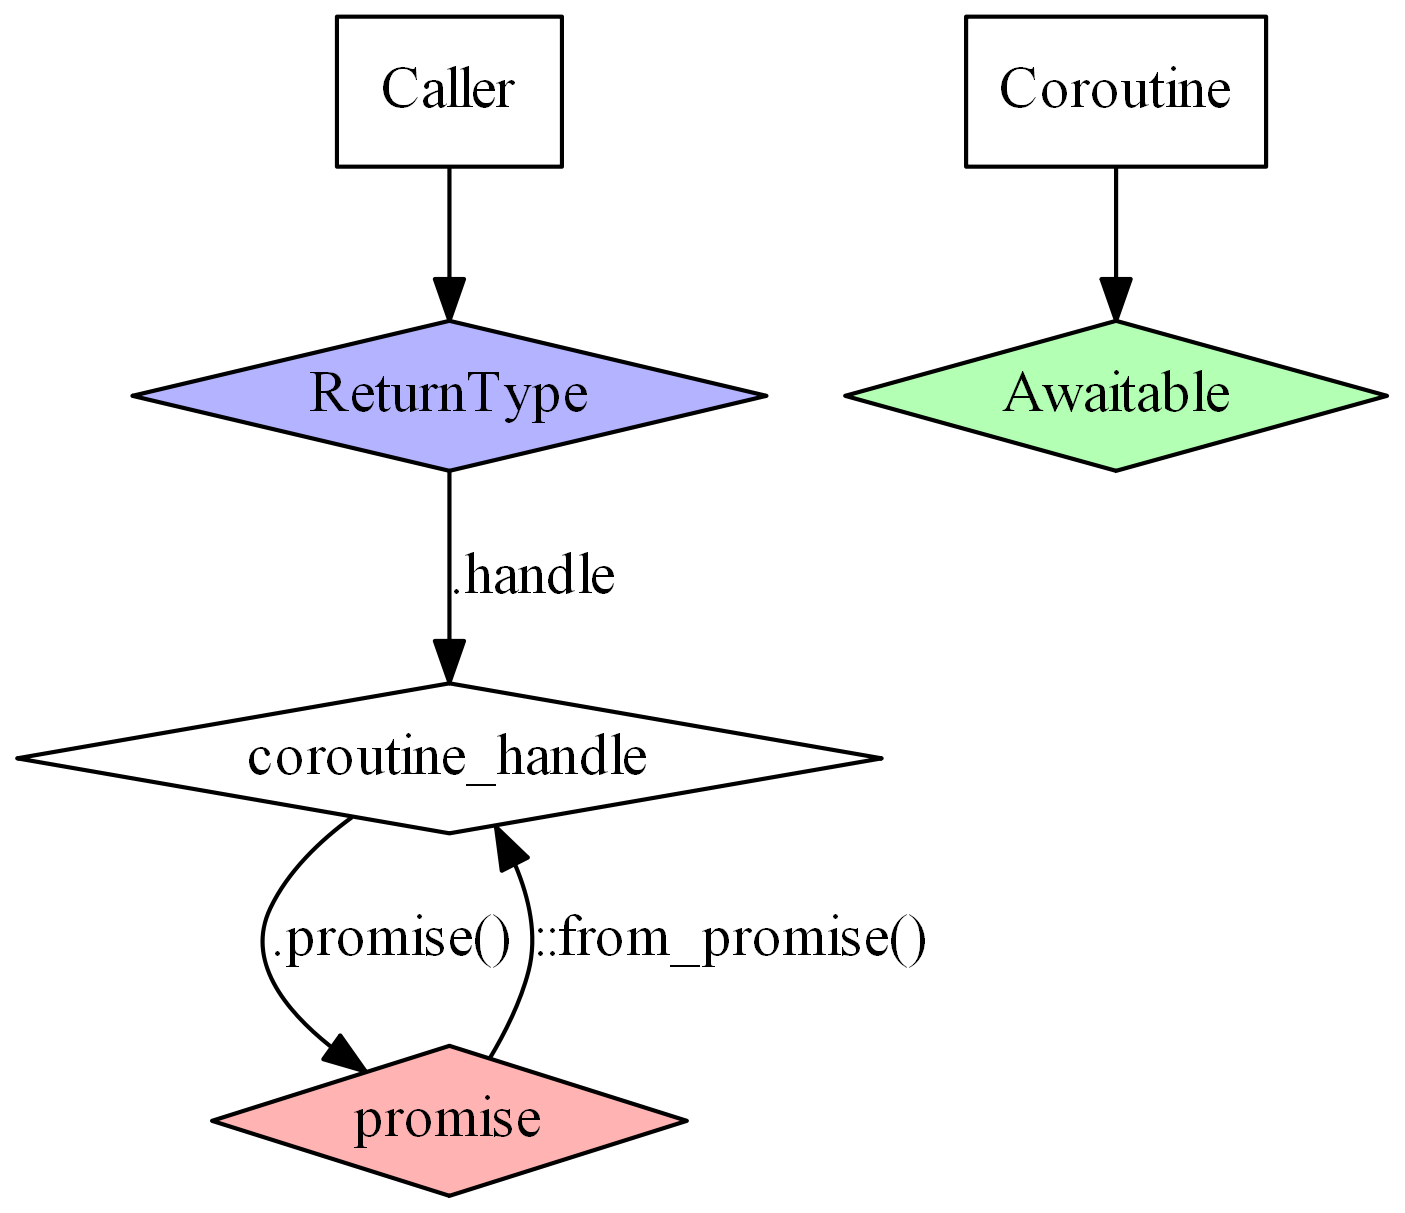
\includegraphics[height=.9\textheight]{corogfx/acquaintances02.png}
  \end{center}
\end{frame}

\begin{frame}[fragile]
  \frametitle{Making acquaintances}

  \begin{lstlisting}[style=cpp20]
struct (*@\tikz[baseline,inner sep=0]\node[anchor=base](ar08){};@*)Awaitable(*@\tikz[baseline,inner sep=0]\node[anchor=base](br08){};@*) {
  void await_suspend(std::coroutine_handle<(*@\tikz[baseline,inner sep=0]\node[anchor=base](cr08){};@*)promise_type(*@\tikz[baseline,inner sep=0]\node[anchor=base](dr08){};@*)>);
};
  \end{lstlisting}
  
  \tikz[overlay]\filldraw[green, opacity=0.3] ([shift={(0,-0.5ex)}]ar08) rectangle ([shift={(0,2ex)}]br08);
  \tikz[overlay]\filldraw[red, opacity=0.3] ([shift={(0,-0.5ex)}]cr08) rectangle ([shift={(0,2ex)}]dr08);
\end{frame}

\begin{frame}[fragile]
  \frametitle{Cheat Sheet: Map of Coroutine Land}
  
  \begin{center}
  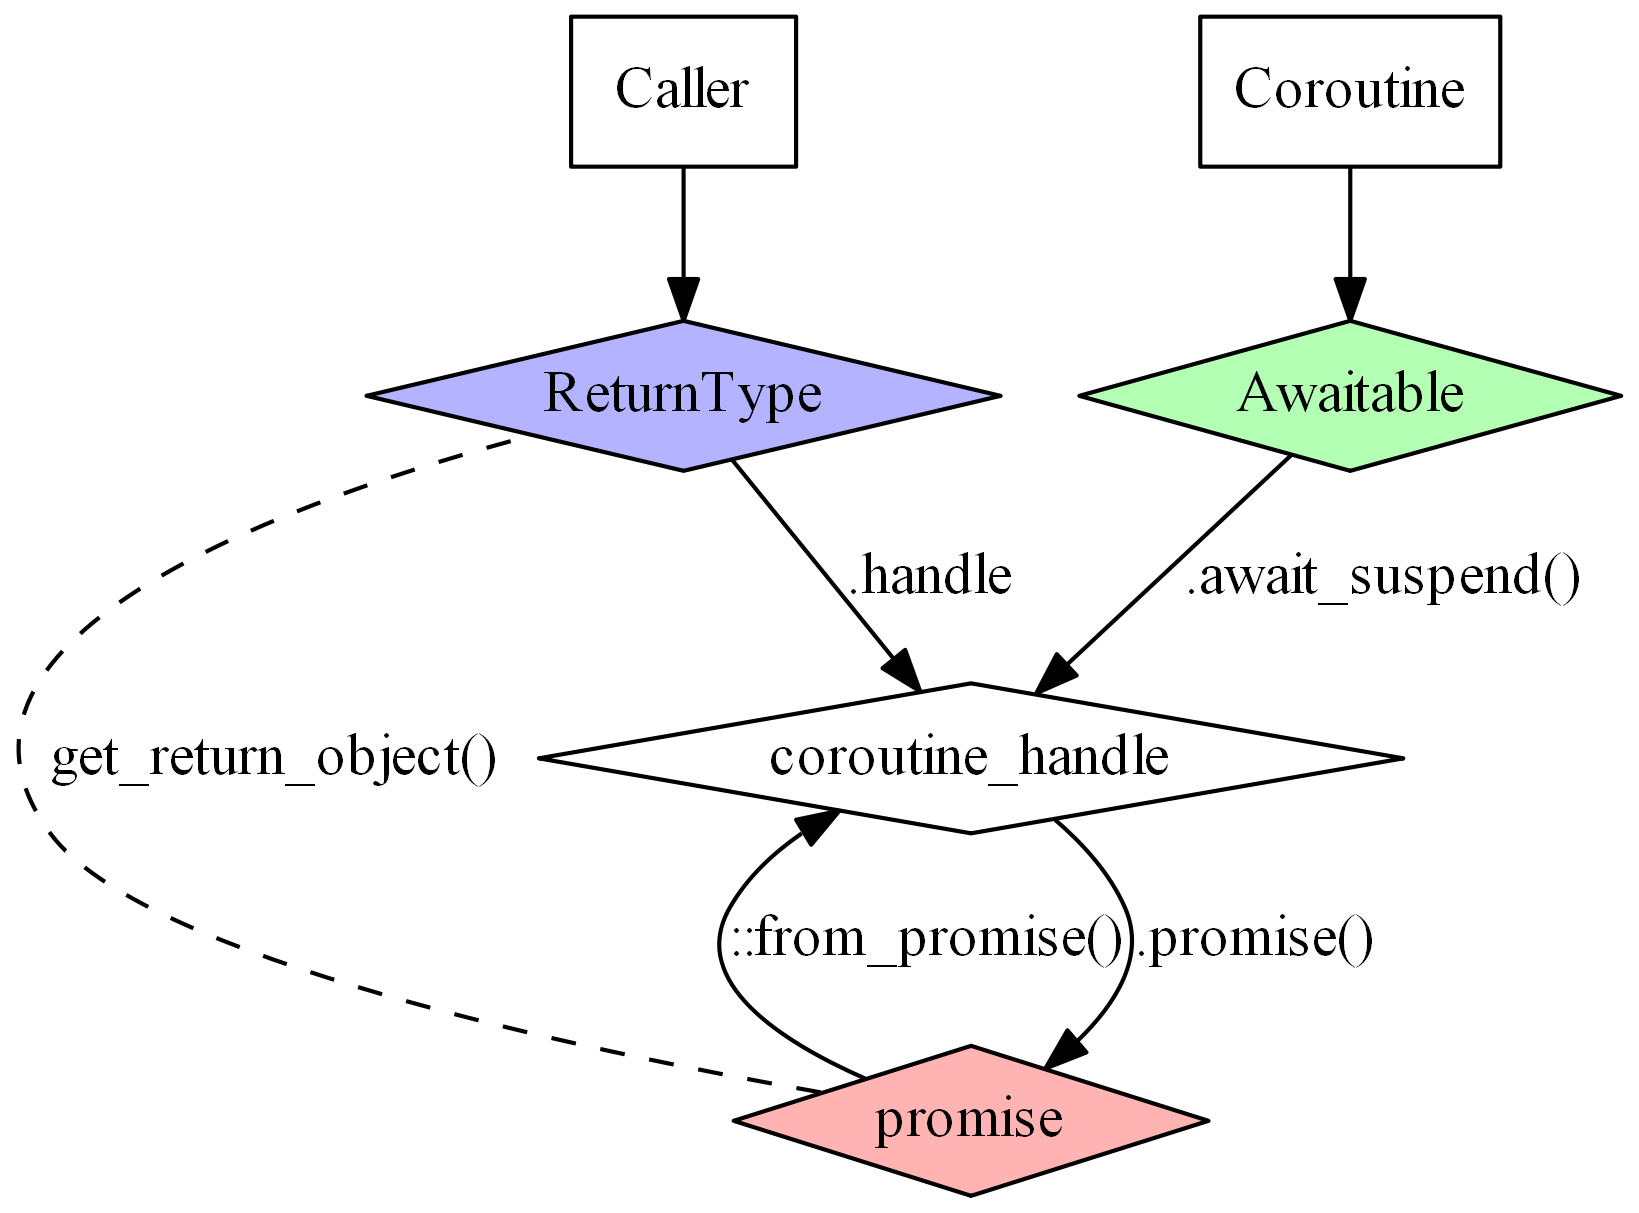
\includegraphics[height=.9\textheight]{corogfx/acquaintances03.png}
  \end{center}
\end{frame}


\begin{frame}[fragile]
  \frametitle{Getting data out of a coroutine}
  \iftransitions \pause \fi
  \begin{center}
  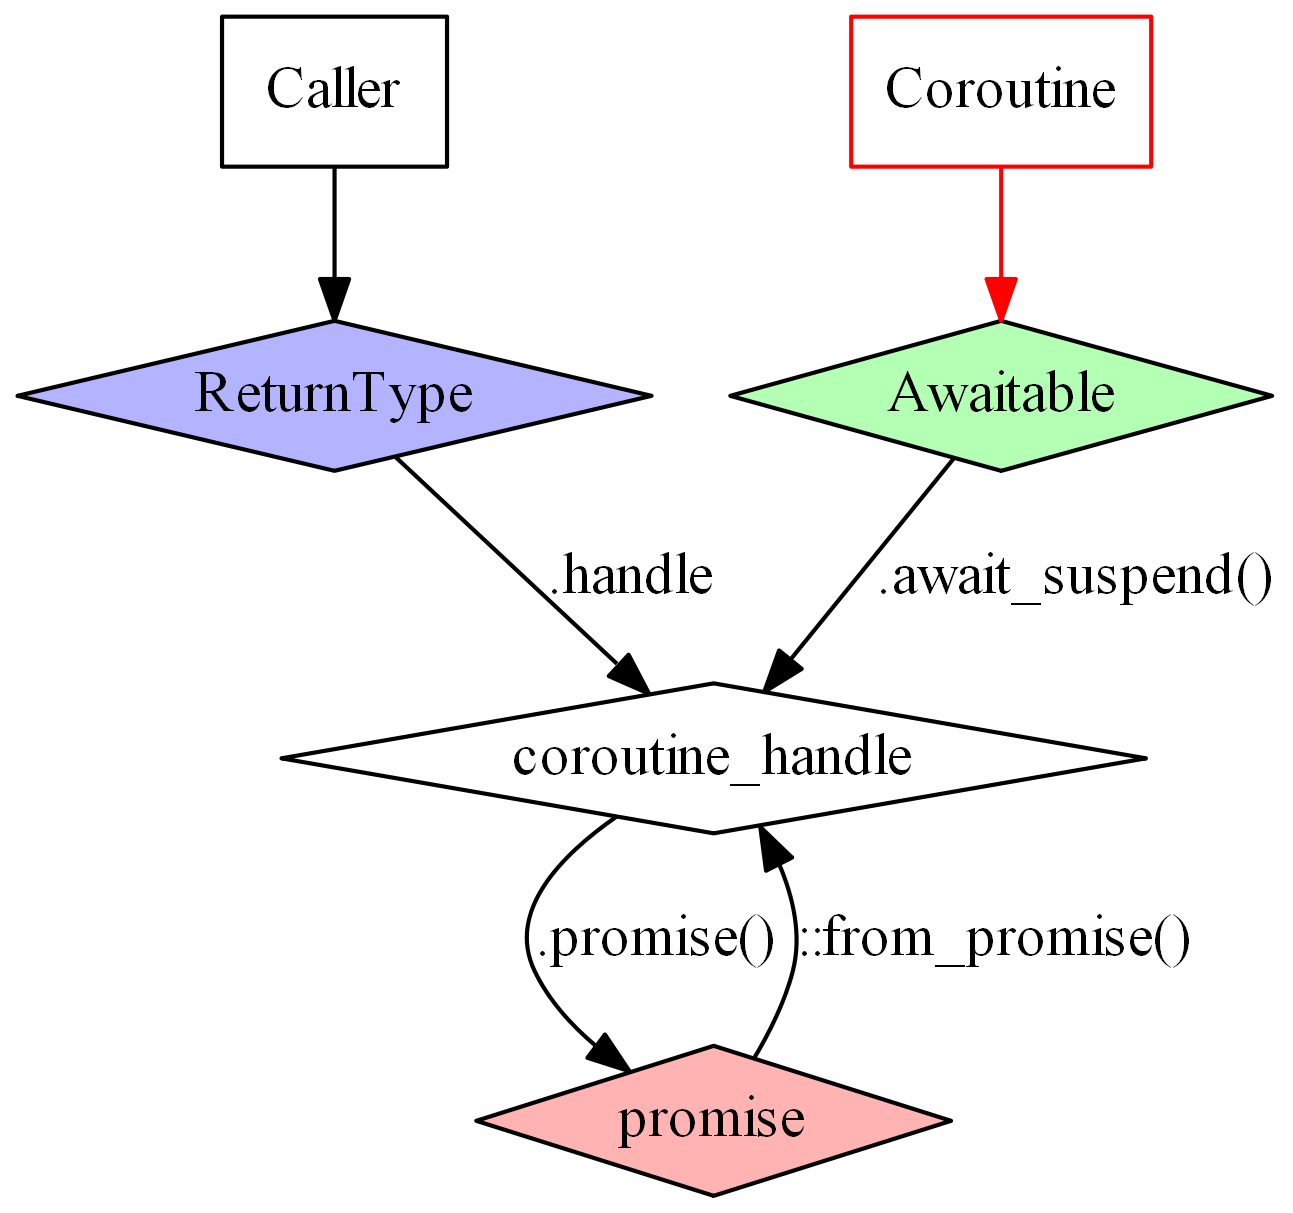
\includegraphics[height=.9\textheight]{corogfx/path_out_010.png}
  \end{center}
  
  \note{Timecheck: 0:40}
\end{frame}

\begin{frame}[fragile]
  \frametitle{Getting data out of a coroutine}
  
  \begin{lstlisting}[language={C++}]
Coroutine f1() {
  // ...
  co_await TheAnswer{42};
}

TheAnswer::TheAnswer(int v)
:value_(v) {}
  \end{lstlisting}
\end{frame}

\begin{frame}[fragile]
  \frametitle{Getting data out of a coroutine}

  \begin{center}
  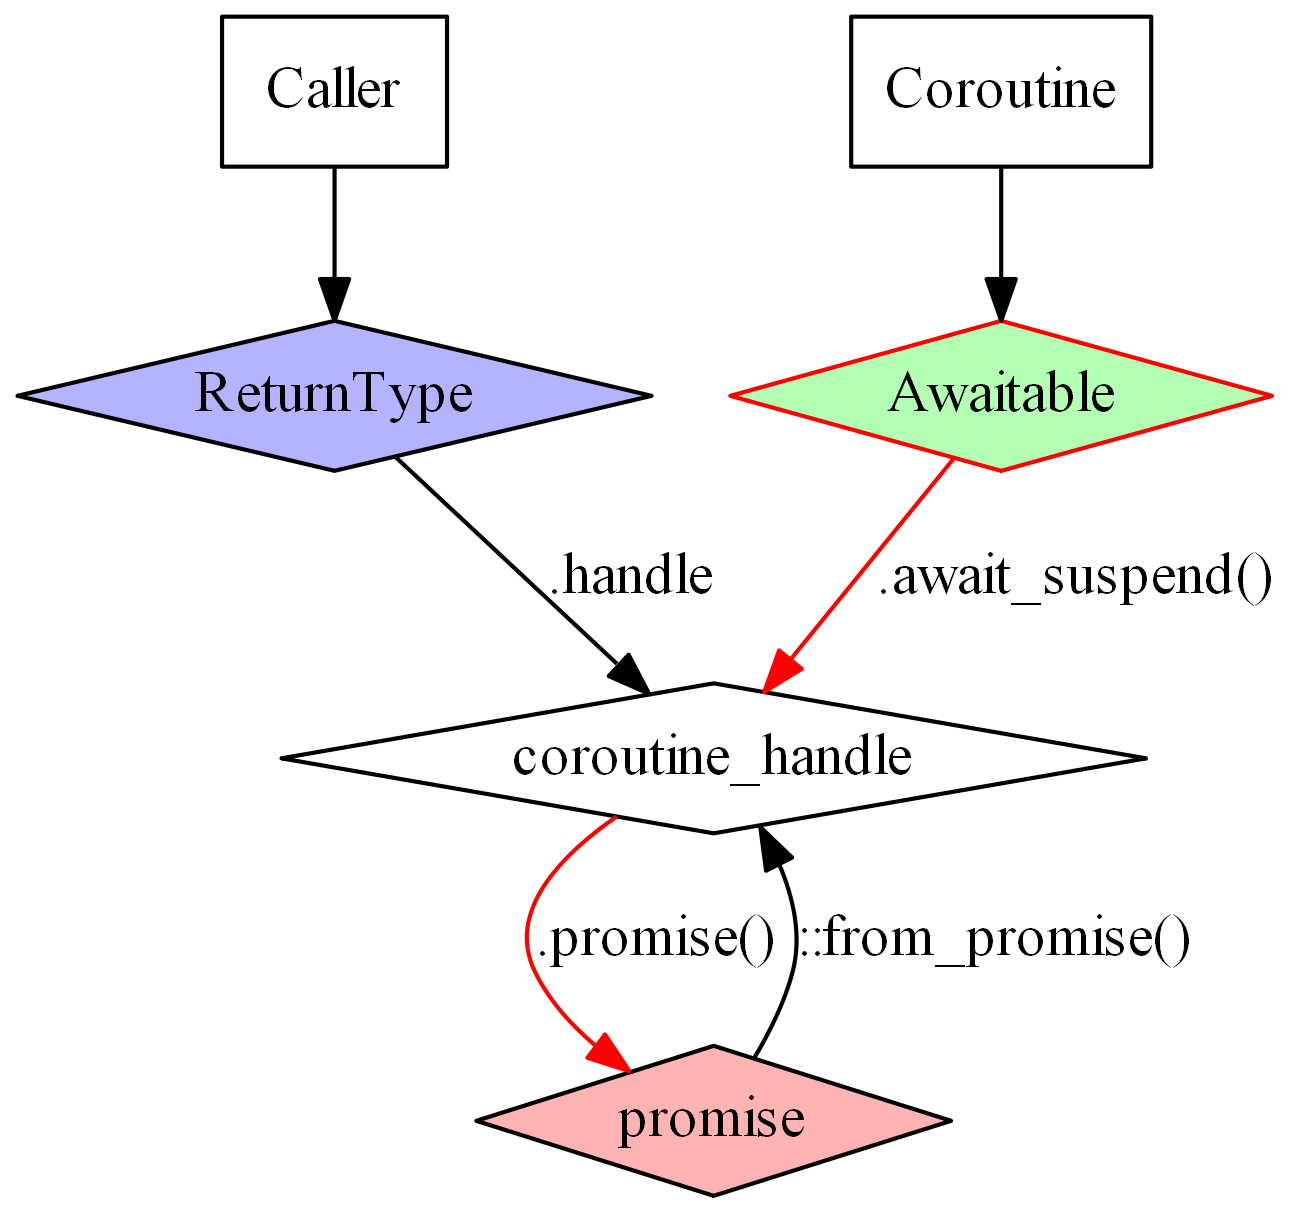
\includegraphics[height=.9\textheight]{corogfx/path_out_020.png}
  \end{center}
\end{frame}

\begin{frame}[fragile]
  \frametitle{Getting data out of a coroutine}
  
  \begin{lstlisting}[language={C++}]
struct promise {
  // ...
  int value;
};

void TheAnswer::await_suspend(
       std::coroutine_handle<promise> h)
{
  h.promise().value = value_;
}
  \end{lstlisting}
\end{frame}

\begin{frame}[fragile]
  \frametitle{Getting data out of a coroutine}

  \begin{center}
  \includegraphics<1>[height=.9\textheight]{corogfx/path_out_030.png}
  \includegraphics<2>[height=.9\textheight]{corogfx/path_out_040.png}
  \end{center}
\end{frame}

\iftransitions
\begin{frame}[fragile]
  \frametitle{Getting data out of a coroutine}
  
  \begin{lstlisting}[language={C++}]
struct Coroutine {
  // ...
  
  
  
  
};
int main() {
  Coroutine c1 = f1();
  std::println("The answer is {}", c1.getAnswer());
}
  \end{lstlisting}
\end{frame} 
\fi

\begin{frame}[fragile]
  \frametitle{Getting data out of a coroutine}
  
  \begin{lstlisting}[language={C++}]
struct Coroutine {
  // ...
  std::coroutine_handle<promise> handle;
  int getAnswer() {
    return handle.promise().value;
  }
};
int main() {
  Coroutine c1 = f1();
  std::println("The answer is {}", c1.getAnswer());
}
  \end{lstlisting}
\end{frame} 

\begin{frame}
  \frametitle{Getting data into a coroutine}
  
  \iftransitions \pause \fi
  
  \begin{center}
  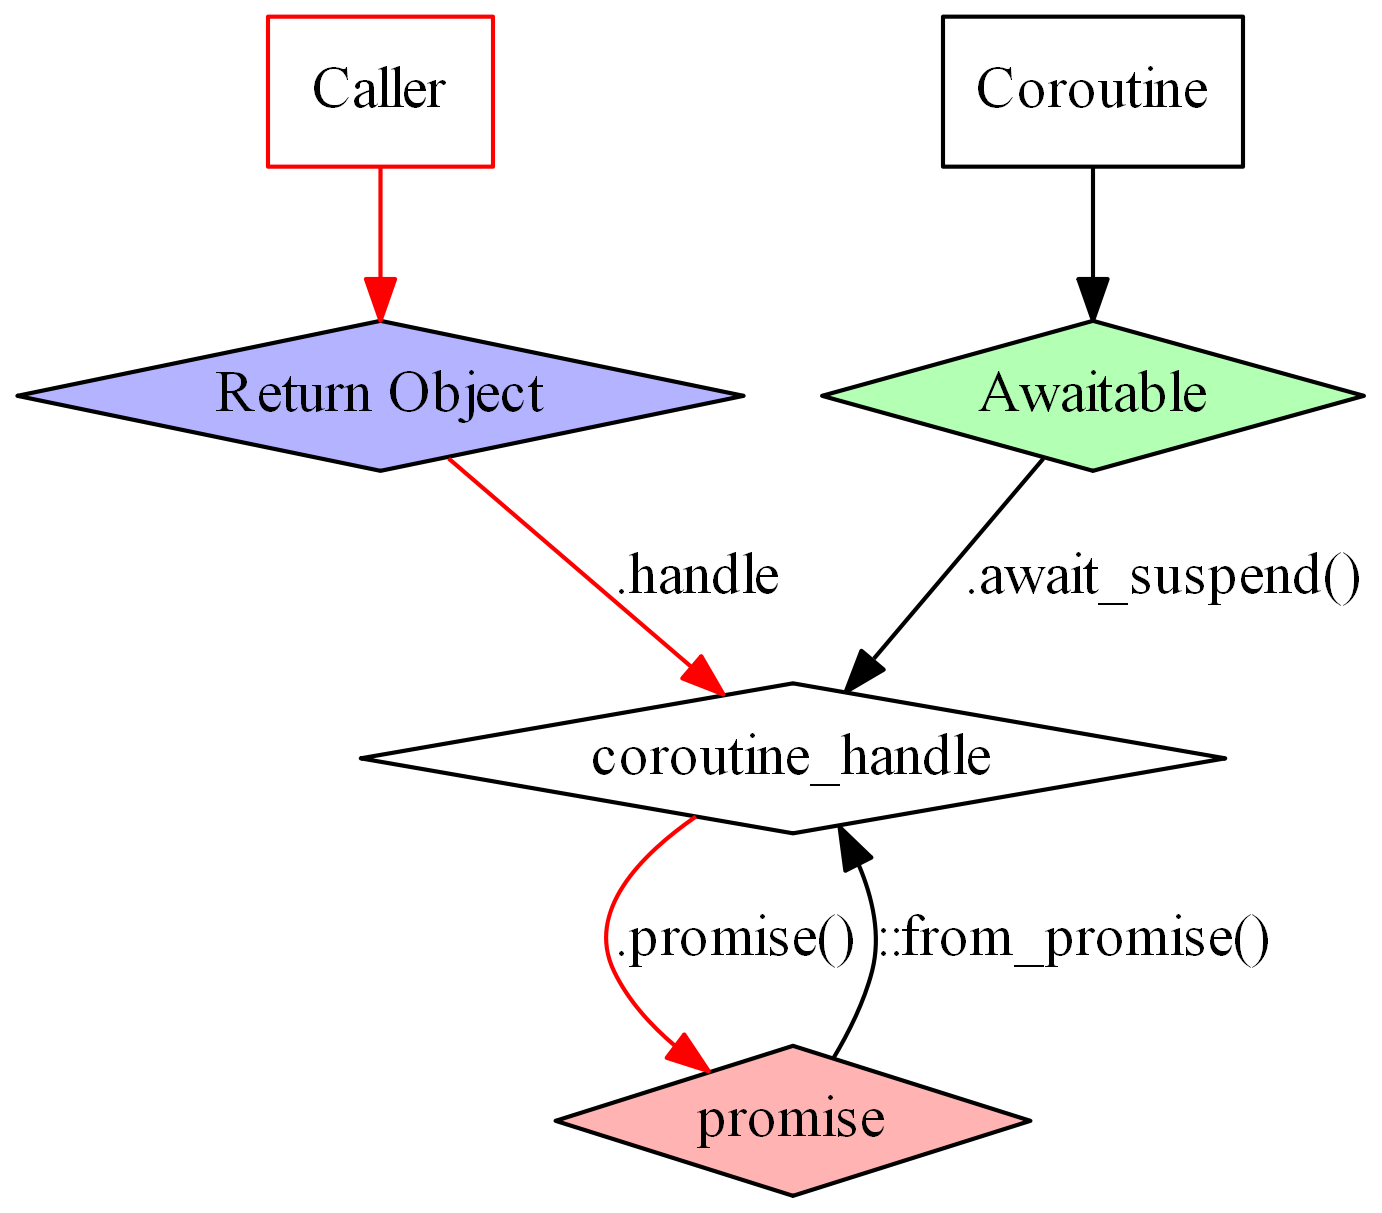
\includegraphics[height=.9\textheight]{corogfx/path_in_010.png}
  \end{center}
  
  \note{Timecheck: 0:46}
\end{frame}

\begin{frame}[fragile]
  \frametitle{Getting data into a coroutine}
  
  \begin{lstlisting}[language={C++}]
Coroutine f1() {
  int the_answer = co_await OutsideAnswer{};
}

int main() {
  Coroutine c1 = f1();
  c1.provide(42);
}
  \end{lstlisting}
\end{frame}

\begin{frame}[fragile]
  \frametitle{Getting data into a coroutine}
  
  \begin{lstlisting}[language={C++}]
void Coroutine::provide(int the_answer) {
  handle.promise().value = the_answer;
  handle.resume();
}
  \end{lstlisting}
\end{frame}

\begin{frame}
  \frametitle{Getting data into a coroutine}
  
  \begin{center}
  \includegraphics<1>[height=.9\textheight]{corogfx/path_in_020.png}
  \includegraphics<2>[height=.9\textheight]{corogfx/path_in_030.png}
  \end{center}
\end{frame}

\iftransitions
\begin{frame}[fragile]
  \frametitle{Getting data into a coroutine}
  
  \begin{lstlisting}[language={C++}]
struct OutsideAnswer {
  bool await_ready() { return false; }
  void await_suspend(std::coroutine_handle<promise> h) {
    handle = h;
  }




  std::coroutine_handle<promise> handle;
};
  \end{lstlisting}
\end{frame}

\fi

\begin{frame}[fragile]
  \frametitle{Getting data into a coroutine}
  
  \begin{lstlisting}[language={C++}]
struct OutsideAnswer {
  bool await_ready() { return false; }
  void await_suspend(std::coroutine_handle<promise> h) {
    handle = h;
  }
  int await_resume() {
    return handle.promise().value;
  }

  std::coroutine_handle<promise> handle;
};
  \end{lstlisting}
\end{frame}

\begin{frame}
  \frametitle{Getting data into a coroutine}
  
  \begin{center}
  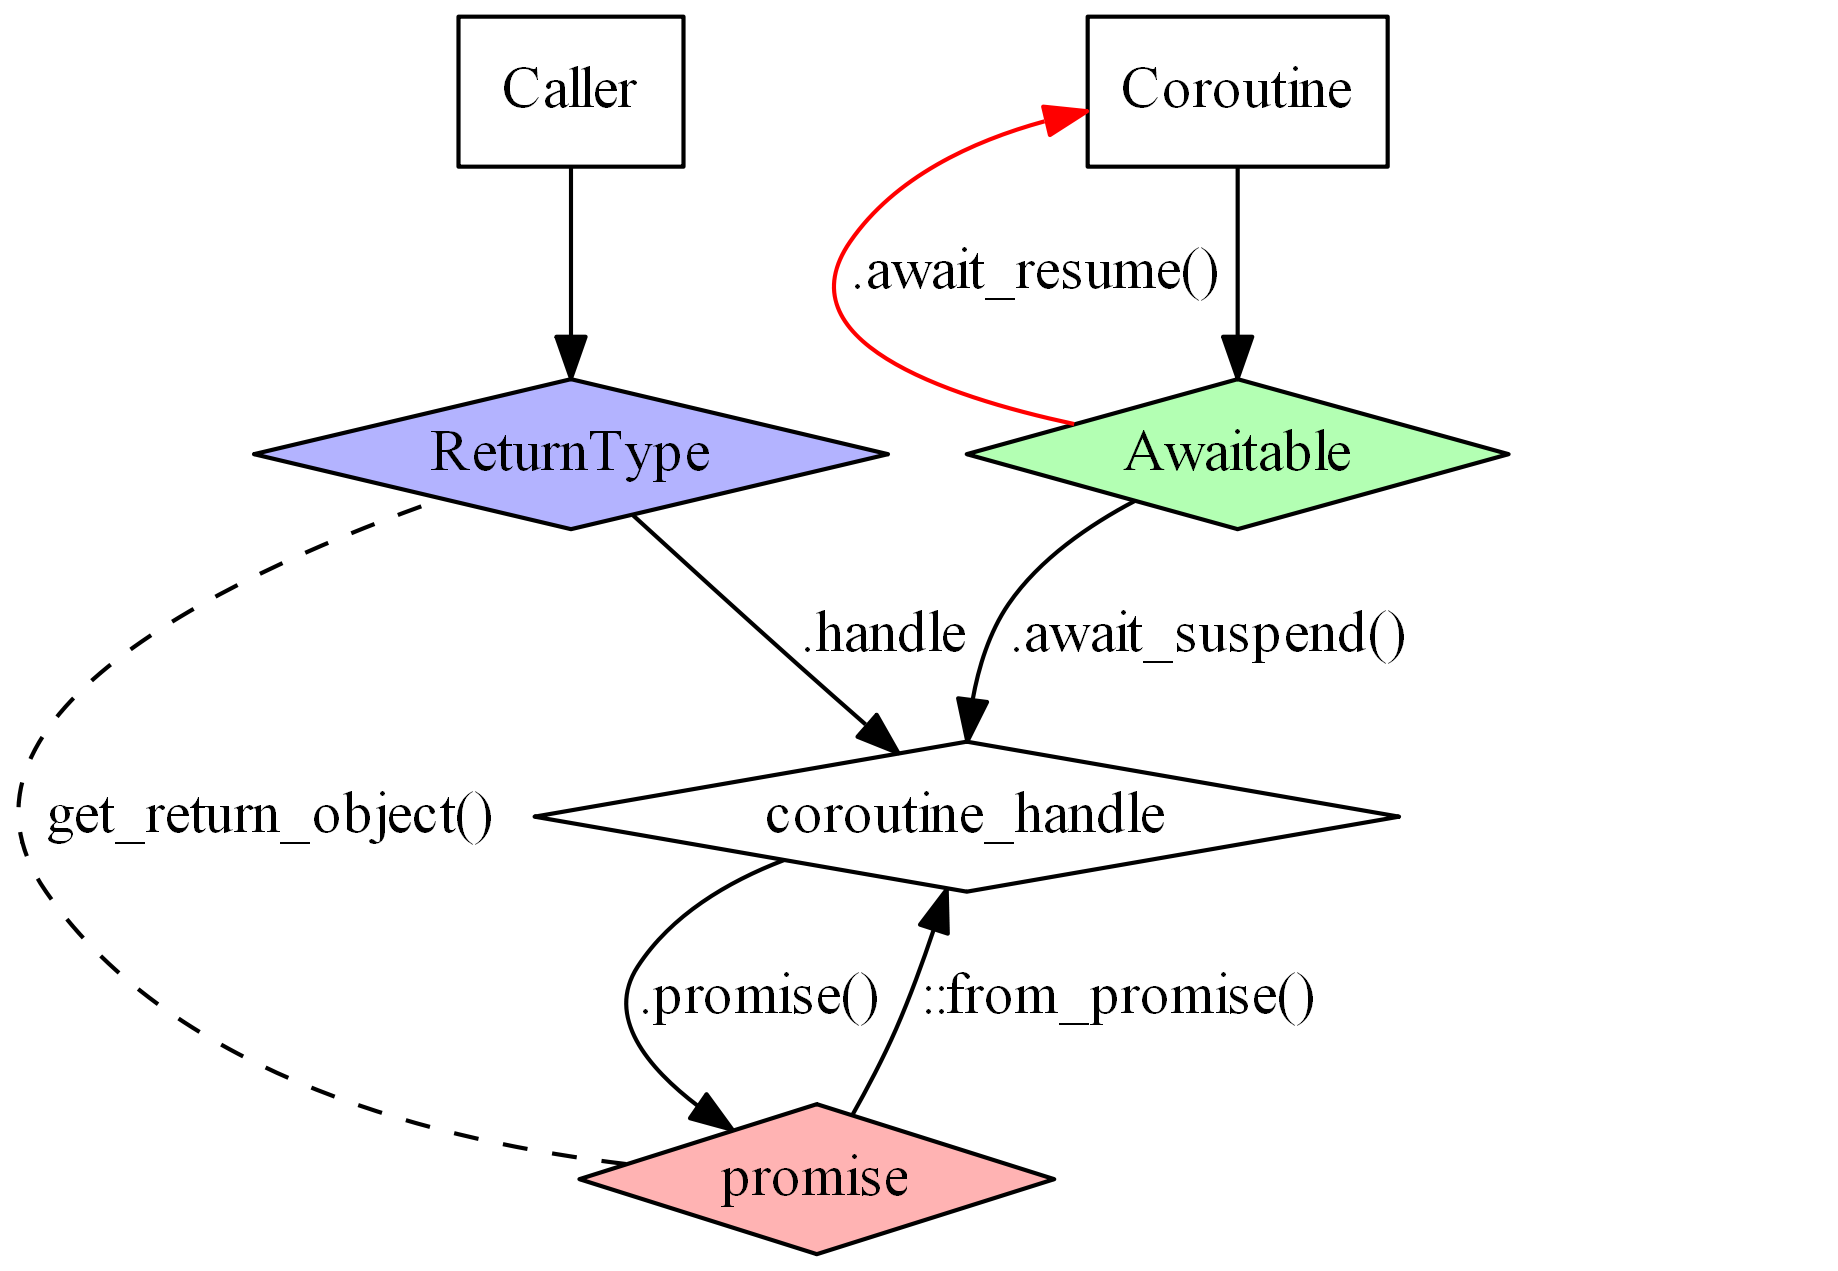
\includegraphics[height=.9\textheight]{corogfx/path_in_040.png}
  \end{center}
\end{frame}


\begin{frame}[fragile]

  \frametitle{Yielding values}

  \begin{lstlisting}[style=cpp20]
FiboGenerator makeFiboGenerator() {
  int i1 = 1;
  int i2 = 1;
  while (;;) {
    co_await NewNumberAwaitable{ i1 };
    i1 = std::exchange(i2, i1 + i2);
  }
}
  \end{lstlisting}

\end{frame}

\begin{frame}[fragile]
  \frametitle{Yielding values}

  \begin{lstlisting}[style=cpp20]
FiboGenerator makeFiboGenerator() {
  int i1 = 1;
  int i2 = 1;
  while (;;) {
    co_yield i1;
    i1 = std::exchange(i2, i1 + i2);
  }
}
  \end{lstlisting}
\end{frame}

\begin{frame}[fragile]
  \frametitle{Yielding values}

  \begin{lstlisting}[style=cpp20]
struct promise_type {
  // ...
  NewNumberAwaitable yield_value(int i) {
    return NewNumberAwaitable{ i };
  }
};
  \end{lstlisting}
\end{frame}

\begin{frame}[fragile]
  \frametitle{Yielding values}

  \begin{lstlisting}[style=cpp20]
struct promise_type {
  // ...
  int value;
  std::suspend_always yield_value(int i) {
    value = i;
    return {};
  }
};
  \end{lstlisting}
\end{frame}

\begin{frame}
  \frametitle{Yielding values}
  \begin{center}
  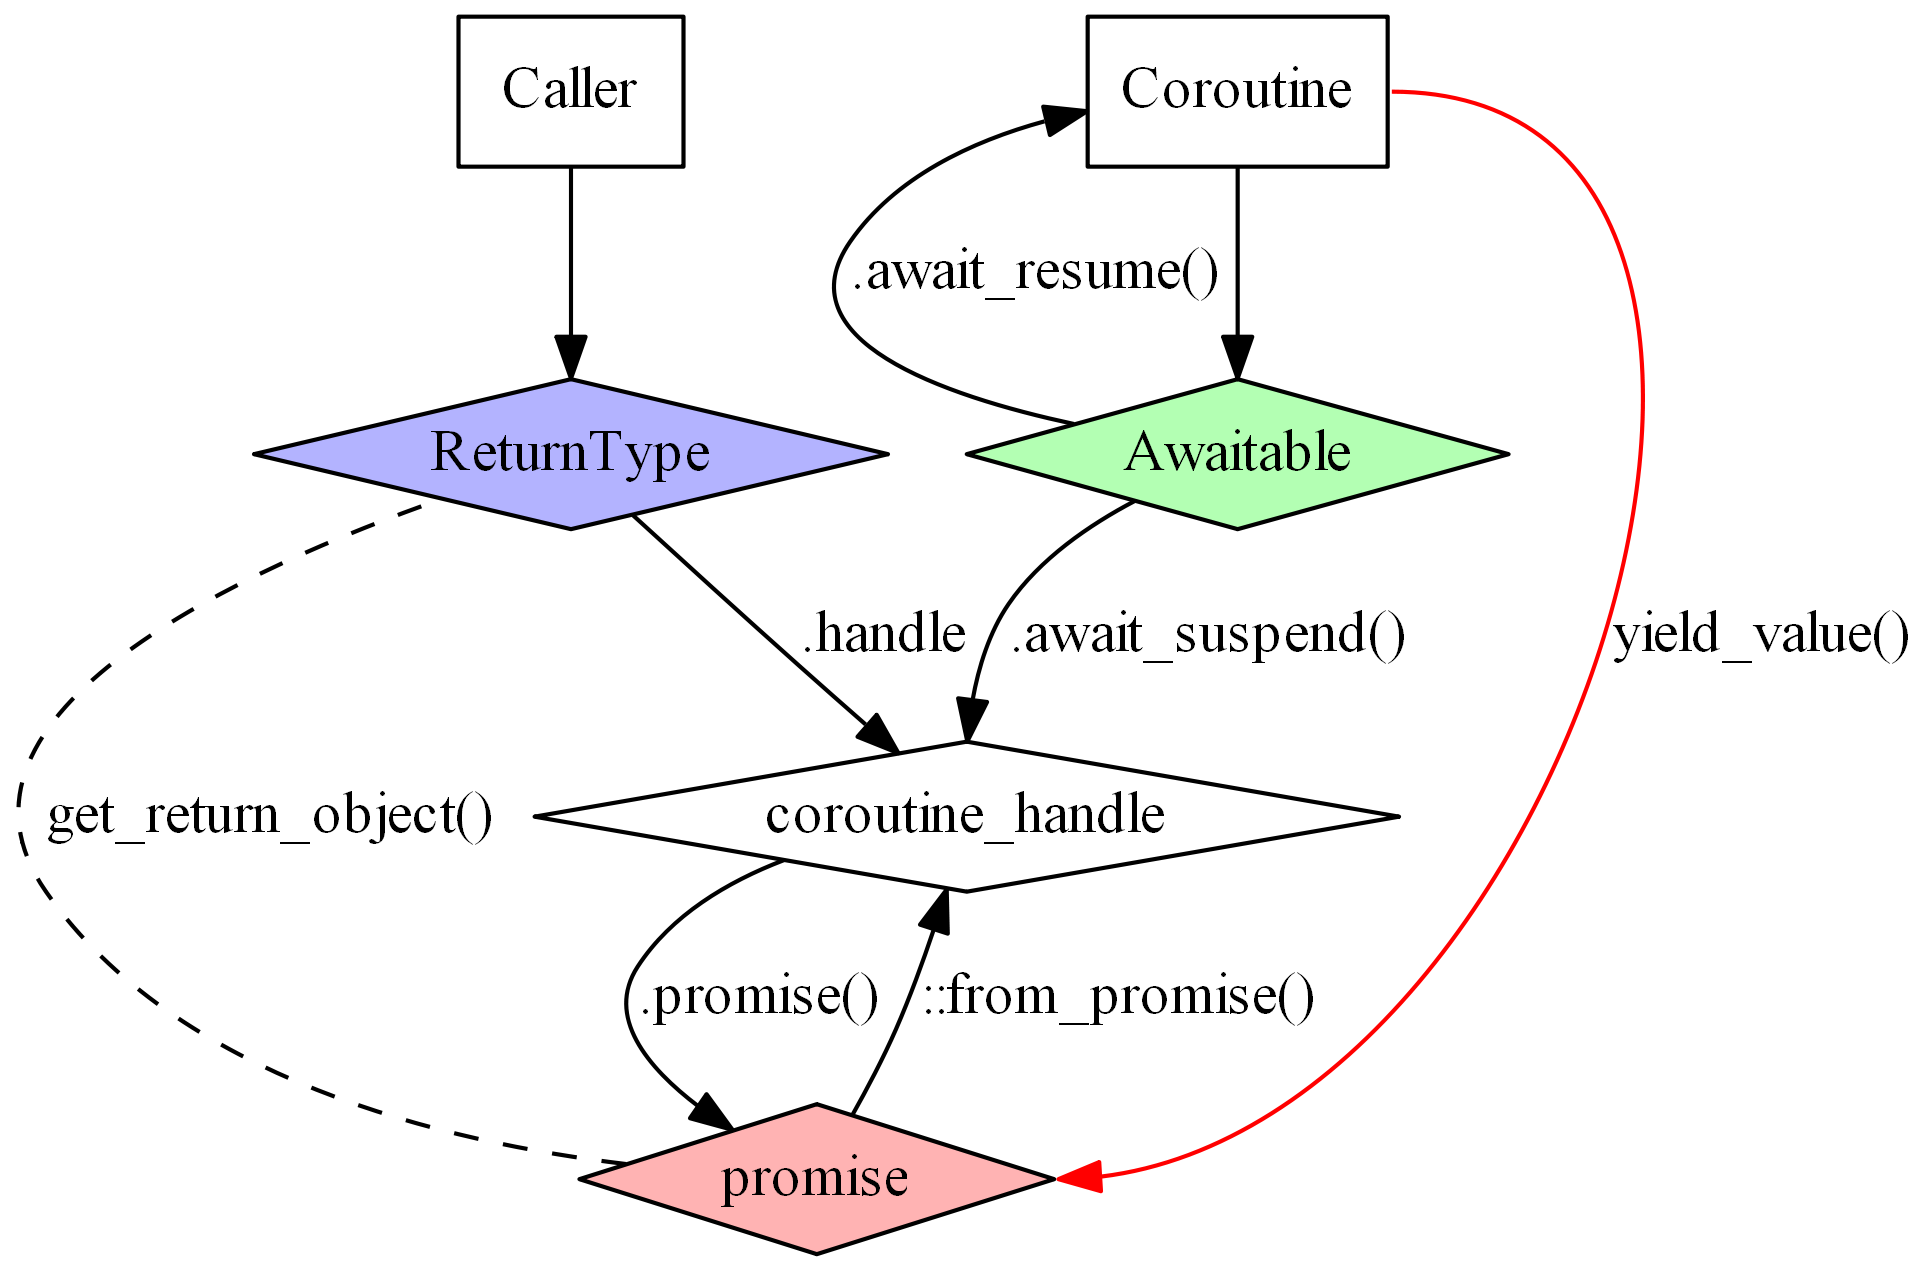
\includegraphics[height=.9\textheight]{corogfx/path_yield_010.png}
  \end{center}
\end{frame}



\iftransitions
\begin{frame}[fragile]
  \frametitle{Symmetric transfer}
  
    \begin{lstlisting}[language={C++}]
co_await Transfer{}; (*@ \iftransitions \pause \fi @*)






std::coroutine_handle<> Transfer::await_suspend(
              std::coroutine_handle<promise> me)
{
  
}
  \end{lstlisting}
\end{frame}
\fi

\begin{frame}[fragile]
  \frametitle{Symmetric transfer}
  
    \begin{lstlisting}[language={C++}]
co_await Transfer{};

struct promise {
  // ...
  std::coroutine_handle<promise> other;
};

std::coroutine_handle<> Transfer::await_suspend(
              std::coroutine_handle<promise> me)
{
  return me.promise().other ? me.promise().other : me;
}
  \end{lstlisting}
  \note{Timecheck: 0:55}
\end{frame}

\begin{frame}
  \frametitle{Wrapping up...}
  
  \note {
  \begin{itemize}
  \item This is all the syntax that you need. Everything else follows from these principles
  \item Learning the syntax was the easy part.  Understanding how to use them is more difficult (but also more fun)
  \item Designing libraries around asynchronous control flow is a very deep topic and hopefully we will see many talks about it in the future
  \item For now hopefully the cheat sheet that we created will help you getting started when picking them up again.
  \end{itemize}
  }
\end{frame}


\begin{frame}[fragile]

  \frametitle{Cheat Sheet - Start/Stop}

  \begin{lstlisting}[style=cpp20,numbers=left]
struct (*@\tikz[baseline,inner sep=0]\node[anchor=base](ar100){};@*)ReturnType(*@\tikz[baseline,inner sep=0]\node[anchor=base](br100){};@*) / std::coroutine_traits<(*@\tikz[baseline,inner sep=0]\node[anchor=base](mr100){};@*)ReturnType(*@\tikz[baseline,inner sep=0]\node[anchor=base](nr100){};@*), ...> { 
  struct (*@\tikz[baseline,inner sep=0]\node[anchor=base](cr100){};@*)promise_type(*@\tikz[baseline,inner sep=0]\node[anchor=base](dr100){};@*) {
    (*@\tikz[baseline,inner sep=0]\node[anchor=base](kr100){};@*)promise_type(T...);(*@\tikz[baseline,inner sep=0]\node[anchor=base](lr100){};@*)  // opt.
    (*@\tikz[baseline,inner sep=0]\node[anchor=base](er100){};@*)ReturnType(*@\tikz[baseline,inner sep=0]\node[anchor=base](fr100){};@*) get_return_object();
    (*@\tikz[baseline,inner sep=0]\node[anchor=base](gr100){};@*)std::suspend_always(*@\tikz[baseline,inner sep=0]\node[anchor=base](hr100){};@*) initial_suspend();
    // ---- (*@$\Uparrow$@*) Start / (*@$\Downarrow$@*) Shutdown ----
    void return_value(T); / void return_void();
    void unhandled_exception();
    (*@\tikz[baseline,inner sep=0]\node[anchor=base](ir100){};@*)std::suspend_always(*@\tikz[baseline,inner sep=0]\node[anchor=base](jr100){};@*) final_suspend() noexcept;
\end{lstlisting}\begin{lstlisting}[style=cpp20]
  };
};
  \end{lstlisting}
  
  \tikz[overlay]\filldraw[blue, opacity=0.3] ([shift={(0,-0.5ex)}]ar100) rectangle ([shift={(0,2ex)}]br100);
  \tikz[overlay]\filldraw[blue, opacity=0.3] ([shift={(0,-0.5ex)}]mr100) rectangle ([shift={(0,2ex)}]nr100);
  \tikz[overlay]\filldraw[red, opacity=0.3] ([shift={(0,-0.5ex)}]cr100) rectangle ([shift={(0,2ex)}]dr100);
  %\tikz[overlay]\filldraw[red, opacity=0.3] ([shift={(0,-0.5ex)}]kr100) rectangle ([shift={(0,2ex)}]lr100);
  \tikz[overlay]\filldraw[blue, opacity=0.3] ([shift={(0,-0.5ex)}]er100) rectangle ([shift={(0,2ex)}]fr100);
  \tikz[overlay]\filldraw[green, opacity=0.3] ([shift={(0,-0.5ex)}]gr100) rectangle ([shift={(0,2ex)}]hr100);
  \tikz[overlay]\filldraw[green, opacity=0.3] ([shift={(0,-0.5ex)}]ir100) rectangle ([shift={(0,2ex)}]jr100);
\end{frame}

\begin{frame}[fragile]

  \frametitle{Cheat Sheet - Awaitable}

  \begin{lstlisting}[style=cpp20,numbers=left]
struct (*@\tikz[baseline,inner sep=0]\node[anchor=base](ar101){};@*)Awaitable(*@\tikz[baseline,inner sep=0]\node[anchor=base](br101){};@*) {
  bool await_ready();
  void await_suspend(std::coroutine_handle <(*@\tikz[baseline,inner sep=0]\node[anchor=base](cr101){};@*)promise_type(*@\tikz[baseline,inner sep=0]\node[anchor=base](dr101){};@*)>);
  void await_resume(); 
};
\end{lstlisting}
  
  \tikz[overlay]\filldraw[green, opacity=0.3] ([shift={(0,-0.5ex)}]ar101) rectangle ([shift={(0,2ex)}]br101);
  \tikz[overlay]\filldraw[red, opacity=0.3] ([shift={(0,-0.5ex)}]cr101) rectangle ([shift={(0,2ex)}]dr101);
\end{frame}

\begin{frame}[fragile]
  \frametitle{Cheat Sheet: Map of Coroutine Land}
  
  \begin{center}
  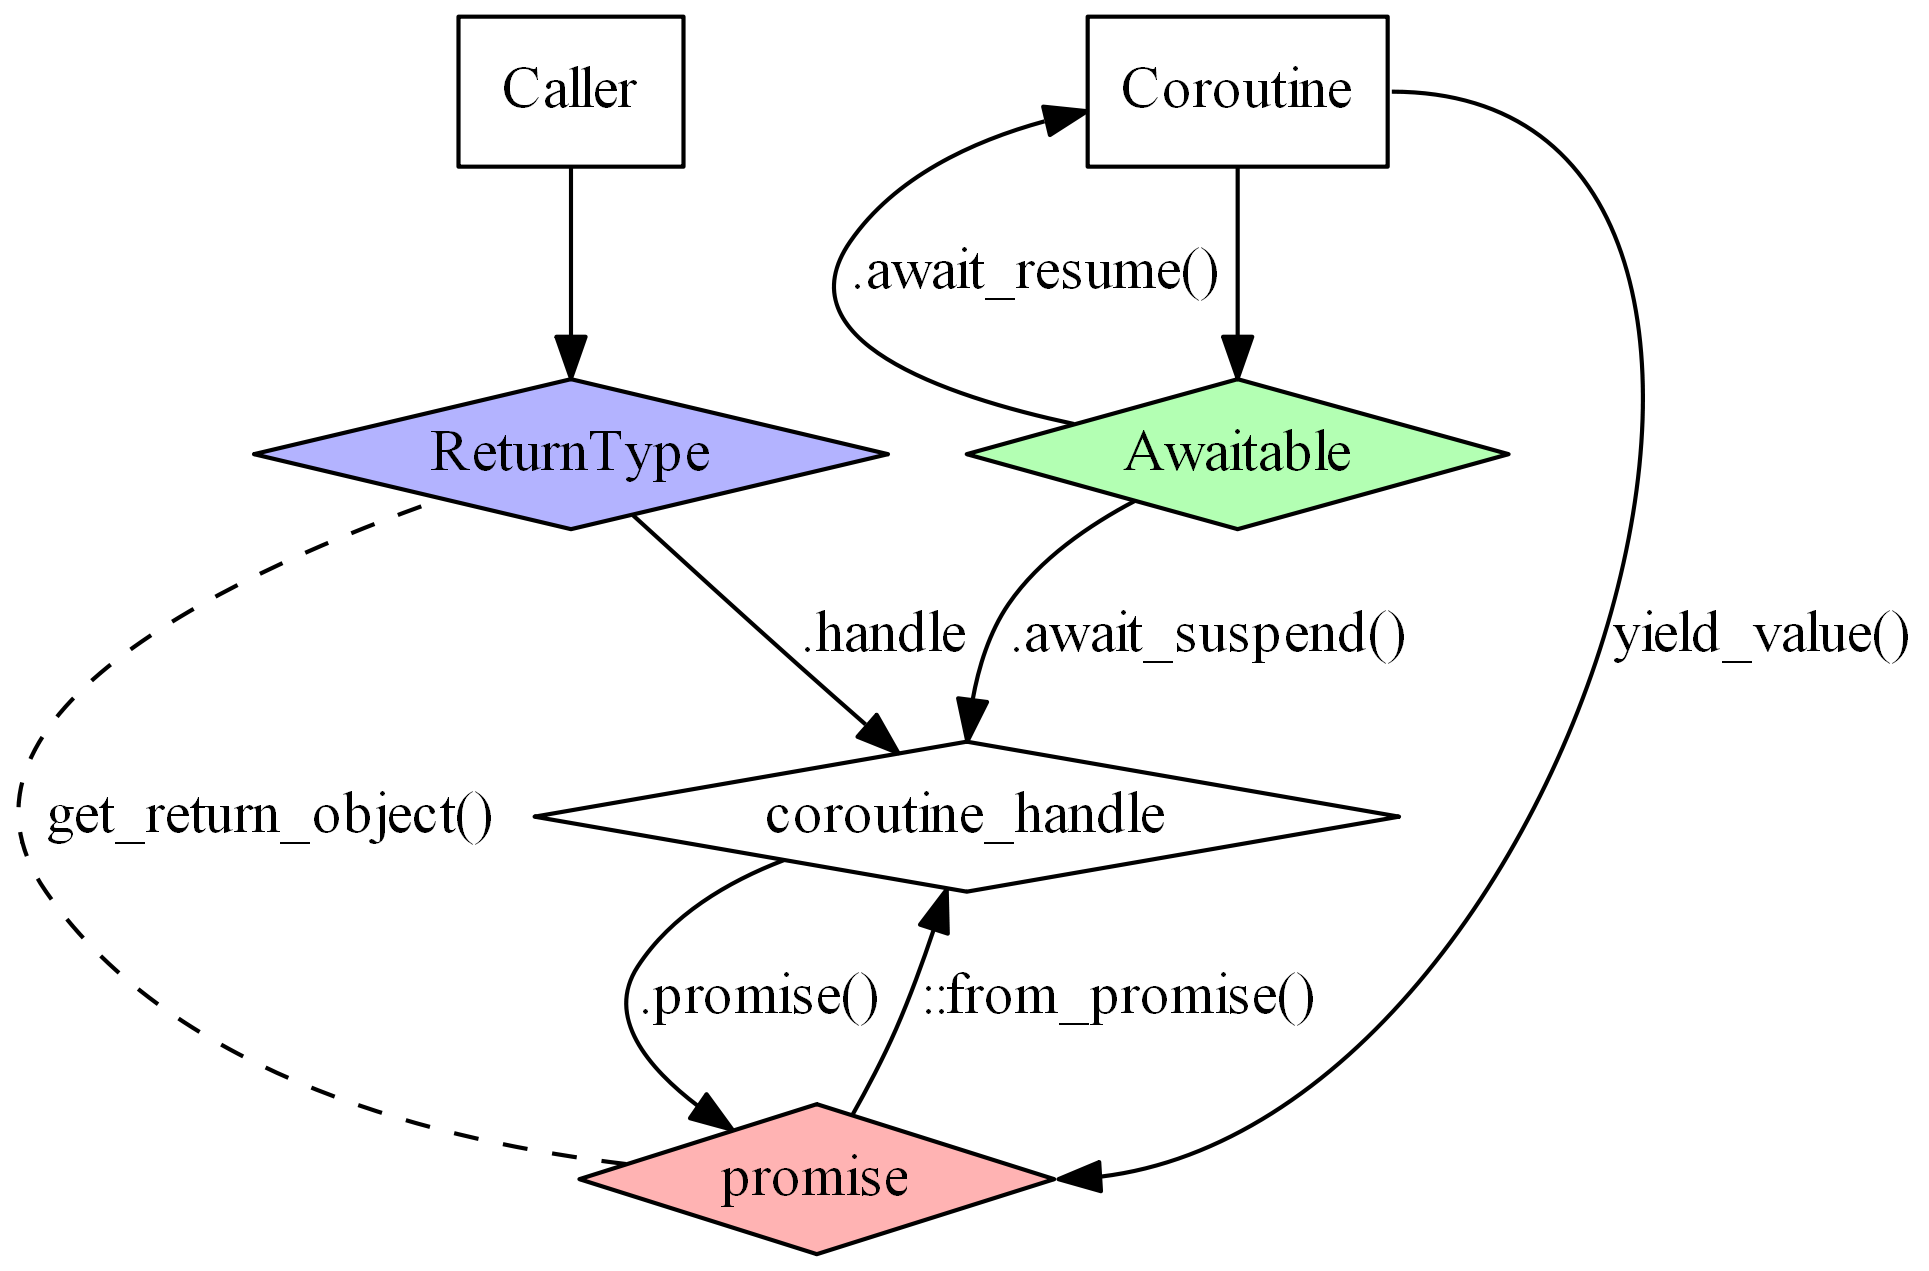
\includegraphics[height=.9\textheight]{corogfx/acquaintances05.png}
  \end{center}
\end{frame}


\begin{frame}
\frametitle{References}
\begin{itemize}
\item \href{https://en.cppreference.com/w/cpp/language/coroutines}{Coroutines on cppreference}
\item \href{https://lewissbaker.github.io/}{Asymmetric Transfer - Lewis Baker's blog on coroutines}
\item \href{https://devblogs.microsoft.com/oldnewthing/}{The Old New Thing - Raymond Chen's blog} \href{https://devblogs.microsoft.com/oldnewthing/20191209-00/?p=103195}{[1]} \href{https://devblogs.microsoft.com/oldnewthing/20210301-00/?p=104914}{[2]}
\end{itemize}

\end{frame}

%\fi %!!!!!!!!!!!!!!!!!

\begin{frame}
  \frametitle{Thanks for your attention.}

  \href{https://stackoverflow.com/users/577603/comicsansms}{
\includegraphics[height=.05\textheight]{resources/so-icon.png}}
  \href{https://github.com/ComicSansMS}{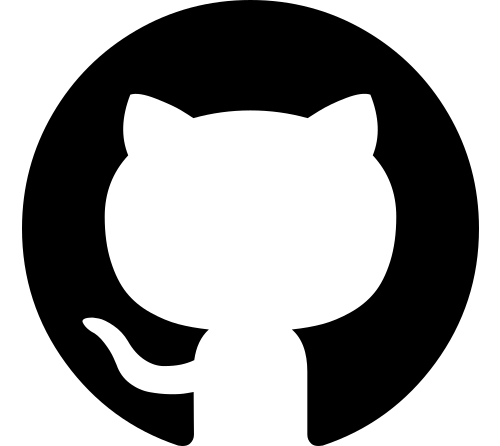
\includegraphics[height=.05\textheight]{resources/github-icon.png}}
  \includegraphics[height=.05\textheight]{resources/discord-icon.png} ComicSansMS /
  \href{https://twitter.com/DerGhulbus/}{
\includegraphics[height=.05\textheight]{resources/twitter-icon.png} @DerGhulbus}

\vspace{20pt}

\begin{center}
  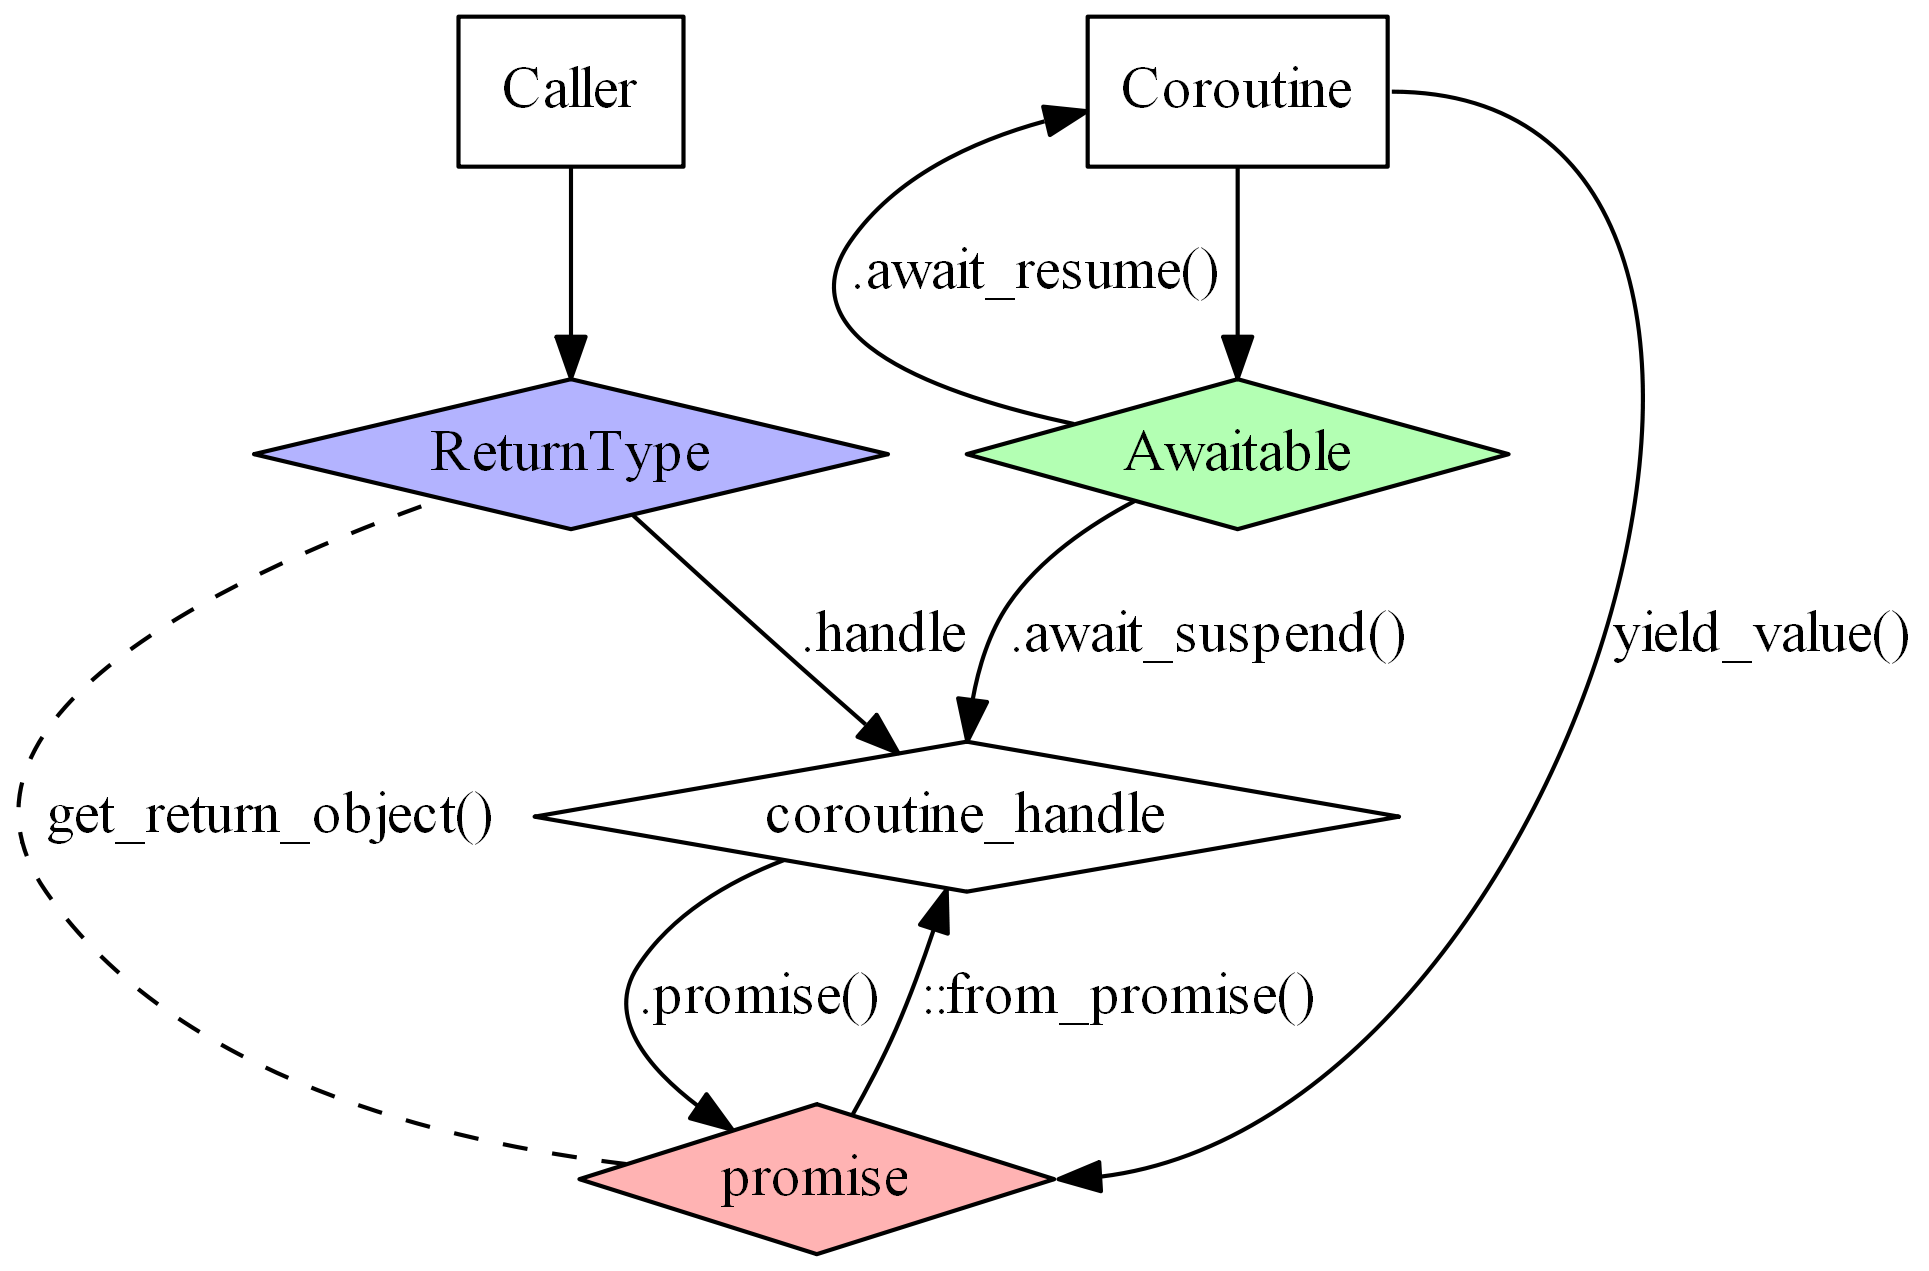
\includegraphics[height=.6\textheight]{corogfx/acquaintances05.png}
  \hspace{12ex}
  \href{https://github.com/ComicSansMS/cpp20_coroutine_cheat_sheet}{\includegraphics[height=.4\textheight]{corogfx/qrcode}}
\end{center}

\end{frame}


\end{document}
